\documentclass[12pt]{article}
\usepackage{fontspec}
\usepackage[margin=2.5cm]{geometry}
\usepackage{amsmath,amssymb}
\usepackage{booktabs,array,longtable,multirow}
\usepackage{graphicx}
\usepackage{float}
\usepackage{caption}
\usepackage{enumitem}
\usepackage[table]{xcolor}
\usepackage{listings}
\usepackage[obeyspaces,spaces]{url}  % keep the spaces inside \path{command args}
\usepackage{pdflscape}
\usepackage{fancyvrb}
\usepackage{tikz}
\usetikzlibrary{shapes.geometric, arrows.meta, positioning}
\usepackage{hyperref}

% สีและรูปทรงของกล่องในผังการทำงาน ใช้ชุดเดียวกับรายงานหลัก
\definecolor{linegrey}{HTML}{94A3B8}
\definecolor{softgrey}{HTML}{F1F5F9}
\definecolor{accentblue}{HTML}{1D4ED8}
\definecolor{normalgreen}{HTML}{15803D}
\definecolor{alertred}{HTML}{B91C1C}
\tikzset{
  box/.style={rectangle, rounded corners=2pt, draw=linegrey, fill=white,
              text width=#1, align=center, inner sep=5pt, font=\small},
  data/.style={box=3.6cm, fill=softgrey},
  proc/.style={box=3.9cm, draw=accentblue, line width=0.7pt},
  outp/.style={box=3.9cm, draw=normalgreen, line width=0.9pt},
  dec/.style={box=4.2cm, draw=alertred, line width=0.9pt},
  ar/.style={-{Stealth[length=2.4mm]}, draw=linegrey, line width=0.8pt},
}

\graphicspath{{./}{githup_manual_figs/}}

\XeTeXlinebreaklocale "th"
\XeTeXlinebreakskip = 0pt plus 1pt
\setmainfont{Angsana New}[Scale=1.15]
\setmonofont{Consolas}[Scale=0.85]

\captionsetup{font=small,labelfont=bf}
\setlength{\parindent}{1.5em}
\setlength{\parskip}{4pt}
\linespread{1.15}

\definecolor{navy}{RGB}{0, 32, 96}
\definecolor{accent}{RGB}{180, 50, 50}
\definecolor{muted}{RGB}{100, 100, 100}

\lstset{
  basicstyle=\ttfamily\small,
  breaklines=true,
  frame=single
}

% หัวข้อเขียนเลขไว้เองในชื่อหัวข้อ จึงใช้แบบมีดอกจัน แล้วต่อท้ายให้เข้าสารบัญเอง
\makeatletter
\let\ews@section\section
\let\ews@subsection\subsection
\newcommand{\ews@sectionstar}[1]{%
  \ews@section*{#1}\phantomsection\addcontentsline{toc}{section}{#1}}
\newcommand{\ews@subsectionstar}[1]{%
  \ews@subsection*{#1}\phantomsection\addcontentsline{toc}{subsection}{#1}}
\renewcommand{\section}{\@ifstar\ews@sectionstar\ews@section}
\renewcommand{\subsection}{\@ifstar\ews@subsectionstar\ews@subsection}
\makeatother
\setcounter{tocdepth}{2}

% กล่องคำสั่ง ใช้รูปแบบเดียวกับรายงานหลัก
\DefineVerbatimEnvironment{Cmd}{Verbatim}{fontsize=\small,frame=single}
\DefineVerbatimEnvironment{CmdS}{Verbatim}{fontsize=\scriptsize,frame=single}

\begin{document}

\begin{center}
{\Large \bfseries คู่มือการติดตั้งและการใช้งานโปรแกรมในคลัง GitHub}\\[4pt]
{\large \bfseries iBond\_LIME, leadning\_time และ ibond\_EWS: โครงสร้างโปรแกรม วิธีติดตั้ง วิธีรัน และผลการรันบน Dataset2}
\end{center}
\vspace{4pt}

\renewcommand{\contentsname}{สารบัญ}
{\makeatletter\let\section\ews@section\tableofcontents\makeatother}
\clearpage

% ====================================================================
\section*{1. วัตถุประสงค์และขอบเขต}

เอกสารนี้เป็นคู่มือการติดตั้งและการรันโปรแกรมในคลัง GitHub สามแห่งของระบบเตือนภัยล่วงหน้าสำหรับหุ้นกู้ภาคเอกชน อธิบายโครงสร้างโปรแกรม วิธีติดตั้ง และวิธีรันทีละคำสั่ง แล้วรายงานผลที่ได้จากการรันจริงบนชุดข้อมูล Dataset2 ทั้งสามคลัง ตาราง~\ref{tab:repos} สรุปหน้าที่ของแต่ละคลัง

\begin{table}[H]
\centering
\small
\caption{คลังโปรแกรมทั้งสามแห่ง}
\label{tab:repos}
\begin{tabular}{@{}p{2.6cm}p{5.2cm}p{6.4cm}@{}}
\toprule
\textbf{คลัง} & \textbf{ที่อยู่} & \textbf{หน้าที่} \\
\midrule
iBond\_LIME & \url{https://github.com/kkabinsky/iBond_LIME} & อธิบายว่าทำไมบริษัทหนึ่งมีค่า PD สูงหรือต่ำ ด้วย LIME และ SHAP พร้อมคิวตรวจแบบ rolling window และ segmented model \\
leadning\_time & \url{https://github.com/kkabinsky/leadning_time} & วัดว่าระบบเตือนก่อนเหตุการณ์จริงได้กี่เดือน (lead time) และจับบริษัทที่เกิดเหตุการณ์ได้กี่ราย \\
ibond\_EWS & \url{https://github.com/kkabinsky/ibond_EWS} & ระบบเตือนภัยเต็มรูปแบบ มีหน้าจอโปรแกรม ค่า PD เส้นเตือนภัย การ shock รายบริษัท และระบบ Dataset2 ในโฟลเดอร์ \path{dataset2/} \\
\bottomrule
\end{tabular}
\end{table}

\textbf{ผลในเอกสารนี้มาจากการรันจริงทุกตัวเลข} ทุกคำสั่งในเอกสารนี้รันบน Dataset2 เมื่อวันที่ 26 กันยายน 2026 บนสำเนาที่ clone ใหม่จากคลัง ไม่ได้รันในโฟลเดอร์ทำงานเดิม เพื่อยืนยันว่าผู้ใช้ที่ได้คลังไปใหม่รันตามคู่มือนี้ได้จริง เครื่องที่ใช้ทดสอบคือ Windows 11 กับ Python 3.14.4 เวลาที่รายงานเป็นเวลาโดยประมาณบนเครื่องนี้ ขณะที่มีงานอื่นรันอยู่ด้วย

\textbf{สามคลังทำงานต่อกันอย่างไร} รูปที่~\ref{fig:repo-flow} แสดงว่าทั้งสามคลังอ่านข้อมูลชุดเดียวกัน แต่ตอบคนละคำถาม ibond\_EWS ให้ค่า PD และเส้นเตือนภัย leadning\_time วัดว่าเส้นเตือนภัยนั้นเตือนได้ทันเวลาหรือไม่ และ iBond\_LIME อธิบายว่าตัวแปรใดทำให้บริษัทนั้นถูกเตือน

\begin{figure}[H]
\centering
\begin{tikzpicture}[node distance=8mm]
\node[data, text width=6.2cm] (d2) {\textbf{Dataset2}\\ \small \path{ibond_33features_panel_941firm}\\ \small 187,007 บริษัท-เดือน 941 บริษัท ตัวแปร 30 ตัว};
\node[proc, below left=12mm and 4mm of d2] (ews) {\textbf{ibond\_EWS}\\ \small PD 3 เดือน เส้นเตือนภัย\\ \small หน้าจอโปรแกรม};
\node[proc, below=12mm of d2] (lead) {\textbf{leadning\_time}\\ \small เตือนก่อนเหตุการณ์\\ \small กี่เดือน จับได้กี่ราย};
\node[proc, below right=12mm and 4mm of d2] (lime) {\textbf{iBond\_LIME}\\ \small ตัวแปรใดดัน PD ขึ้น\\ \small LIME และ SHAP};
\node[outp, below=12mm of lead, text width=9.0cm] (out) {ผลลัพธ์: ตาราง CSV, Excel, ฐานข้อมูล SQLite, รูป JPG/PNG และหน้าจอโปรแกรม};
\draw[ar] (d2) -- (ews);
\draw[ar] (d2) -- (lead);
\draw[ar] (d2) -- (lime);
\draw[ar] (ews) -- (out);
\draw[ar] (lead) -- (out);
\draw[ar] (lime) -- (out);
\end{tikzpicture}
\caption{ความสัมพันธ์ของคลังทั้งสามแห่งกับข้อมูล Dataset2}
\label{fig:repo-flow}
\end{figure}

\textbf{ลำดับของเอกสาร} หัวข้อที่ 2 อธิบายข้อมูล หัวข้อที่ 3 อธิบายการติดตั้งที่ใช้ร่วมกันทั้งสามคลัง หัวข้อที่ 4 ถึง 6 เป็นคู่มือของแต่ละคลัง เรียงจากโครงสร้างโปรแกรม วิธีรัน ไปจนถึงผลที่ได้ หัวข้อที่ 7 สรุปสิ่งที่ปรับปรุงในคลังรอบนี้และข้อควรทราบ ส่วนภาคผนวก ก รวมคำสั่งทั้งหมดไว้ในหน้าเดียว

% ====================================================================
\section*{2. ข้อมูล Dataset2}

ทั้งสามคลังใช้ตาราง \path{ibond_33features_panel_941firm} เป็นข้อมูลหลัก ตาราง~\ref{tab:d2} สรุปตัวเลขสำคัญ ทุกตัวเลขนับจากตารางจริงด้วยคำสั่ง \path{inspect} ของโปรแกรมคำนวณ lead time

\begin{table}[H]
\centering
\small
\caption{ตัวเลขหลักของ Dataset2}
\label{tab:d2}
\begin{tabular}{@{}lp{9.4cm}@{}}
\toprule
\textbf{รายการ} & \textbf{ค่า} \\
\midrule
ชื่อตาราง & \path{ibond_33features_panel_941firm} \\
บริษัท-เดือน & 187,007 แถว 95 คอลัมน์ \\
บริษัท & 941 ราย ทั้งตลาด SET และ mai \\
ช่วงเวลา & 1984-01 ถึง 2026-08 \\
ตัวแปรที่เข้าแบบจำลอง & 30 ตัว (ตาราง~\ref{tab:features}) \\
ตัวแปรตาม & \path{y_pre3m} เท่ากับ 1 เมื่อบริษัทผิดนัดชำระหนี้หรือปรับโครงสร้างหนี้จริงภายในเดือนนี้ถึงสามเดือนข้างหน้า \\
เดือนที่ \path{y_pre3m} = 1 & 124 เดือน จาก 31 บริษัท คิดเป็นร้อยละ 0.066 \\
บริษัทที่เกิดเหตุการณ์ & 32 ราย โดย 31 รายมีเดือนเริ่มเหตุการณ์ชัดเจน อีก 1 รายทราบจากคอลัมน์สถานะเท่านั้น \\
\bottomrule
\end{tabular}
\end{table}

\begin{table}[H]
\centering
\small
\caption{ตัวแปร 30 ตัวที่เข้าแบบจำลอง แบ่งเป็นห้ากลุ่ม}
\label{tab:features}
\begin{tabular}{@{}p{3.6cm}p{10.6cm}@{}}
\toprule
\textbf{กลุ่ม} & \textbf{ตัวแปร} \\
\midrule
สภาพคล่องการซื้อขาย (5) & \path{amihud_monthly}, \path{adj_illiq_kz}, \path{percent_zero_days}, \path{zero_days}, \path{n_days} \\
อัตราส่วนทางการเงิน (14) & \path{ROA}, \path{ROE}, \path{DE}, \path{CurrentRatio}, \path{QuickRatio}, \path{CashRatio}, \path{EBITtoTA}, \path{REtoTA}, \path{WorkingCapitaltoTA}, \path{TDTA}, \path{LTDtoTA}, \path{STDtoTA}, \path{cf_Interestcoverageratio}, \path{acc_DebtServiceCoverageRatio} \\
ขนาดและอายุ (2) & \path{lnTotalAssets}, \path{lnAge} \\
เศรษฐกิจมหภาค (3) & \path{Policyrate}, \path{GDPgrowth}, \path{UnemploymentratemodeledILOe} \\
ธรรมาภิบาลและ ESG (6) & \path{ESGScore}, \path{GovernancePillarScore}, \path{EnvironmentalPillarScore}, \path{SocialPillarScore}, \path{IndependentBoardMembers}, \path{AverageBoardTenure} \\
\bottomrule
\end{tabular}
\end{table}

\textbf{ข้อมูลอยู่ที่ไหนในแต่ละคลัง} ทั้งสามคลังแนบ Dataset2 มาในตัว ผู้ใช้จึงไม่ต้องหาฐานข้อมูลเอง ตาราง~\ref{tab:data-where} บอกว่าแต่ละคลังเก็บไว้ในรูปใด และโปรแกรมเปิดใช้อย่างไร

\begin{table}[H]
\centering
\small
\caption{ตำแหน่งของ Dataset2 ในแต่ละคลัง}
\label{tab:data-where}
\begin{tabular}{@{}p{2.4cm}p{4.6cm}p{7.2cm}@{}}
\toprule
\textbf{คลัง} & \textbf{ไฟล์ที่แนบมา} & \textbf{โปรแกรมเปิดใช้อย่างไร} \\
\midrule
iBond\_LIME & \path{lime_credit.db.zip} (23.9 MB) & คลายซิปเองเป็น \path{lime_credit.db} (121 MB) ในการรันครั้งแรก \\
leadning\_time & \path{lime_credit.db.zip} (ไฟล์เดียวกัน) & คลายซิปเองในการรันครั้งแรกเช่นกัน \\
ibond\_EWS & \path{dataset/ibond_33features_panel_941firm.csv.gz} (17.3 MB) & สั่ง \path{python dataset/build_db.py} ครั้งเดียว ได้ \path{cmdf_credit.db} (109.5 MB) ที่รากของคลัง \\
\bottomrule
\end{tabular}
\end{table}

\textbf{ตรวจแล้วว่าข้อมูลทั้งสามแห่งเป็นชุดเดียวกัน} ตาราง Dataset2 ในฐานข้อมูลทำงานเดิม \path{cmdf_credit.db} กับใน \path{lime_credit.db} ให้ค่า hash เดียวกันเมื่อคำนวณจากทั้ง 95 คอลัมน์ ส่วนฐานข้อมูลที่ ibond\_EWS สร้างกลับจากไฟล์ CSV ให้ตัวแปรเข้าแบบจำลองตรงกันทุกค่า ผลต่างสูงสุดเป็นศูนย์ ตัวแปรตามตรงกันทุกแถว และบัญชีเหตุการณ์ 31 และ 32 รายตรงกัน ดังนั้นตัวเลขที่ได้จากคลังใดก็ตาม เทียบกันได้โดยตรง

% ====================================================================
\section*{3. การติดตั้ง}

\subsection*{3.1 สิ่งที่ต้องมี}

\begin{itemize}[leftmargin=1.6em, itemsep=2pt]
\item Python 3.10 ขึ้นไป เครื่องทดสอบใช้ 3.14.4
\item git สำหรับ clone คลัง หรือดาวน์โหลดเป็นไฟล์ zip จากหน้า GitHub ก็ได้
\item พื้นที่ว่างราว 1 GB สำหรับฐานข้อมูลที่คลายแล้วและผลการรัน
\item XeLaTeX และฟอนต์ Angsana New เฉพาะกรณีต้องการคอมไพล์คู่มือนี้ใหม่
\end{itemize}

ตาราง~\ref{tab:versions} คือรุ่นของแพ็กเกจบนเครื่องที่ใช้ทดสอบ รุ่นที่ใหม่กว่านี้ควรใช้ได้ แต่ถ้าต้องการผลตรงกับเอกสารนี้ทุกตัวเลข ควรใช้รุ่นเดียวกัน

\begin{table}[H]
\centering
\small
\caption{รุ่นของแพ็กเกจที่ใช้ทดสอบ}
\label{tab:versions}
\begin{tabular}{@{}llll@{}}
\toprule
\textbf{แพ็กเกจ} & \textbf{รุ่น} & \textbf{แพ็กเกจ} & \textbf{รุ่น} \\
\midrule
numpy & 2.4.4 & catboost & 1.2.10 \\
pandas & 3.0.2 & lightgbm & 4.6.0 \\
scikit-learn & 1.8.0 & lime & 0.2.0.1 \\
scipy & 1.17.1 & shap & 0.52.0 \\
xgboost & 3.2.0 & statsmodels & 0.14.6 \\
matplotlib & 3.10.8 & flet & 0.84.0 \\
openpyxl & 3.1.5 & xlsxwriter & 3.2.9 \\
Pillow & 12.2.0 & & \\
\bottomrule
\end{tabular}
\end{table}

\subsection*{3.2 ดาวน์โหลดคลัง}

วางทั้งสามคลังไว้ในโฟลเดอร์เดียวกัน เช่น \path{D:\work} แต่ละคลังทำงานแยกกันได้ ไม่ต้องอยู่ติดกัน

\begin{Cmd}
cd D:\work
git clone https://github.com/kkabinsky/iBond_LIME.git
git clone https://github.com/kkabinsky/leadning_time.git
git clone https://github.com/kkabinsky/ibond_EWS.git
\end{Cmd}

\subsection*{3.3 ติดตั้งแพ็กเกจ}

แนะนำให้สร้าง virtual environment ก่อน แล้วติดตั้งตามไฟล์ requirements ของแต่ละคลัง

\begin{Cmd}
python -m venv .venv
.\.venv\Scripts\Activate.ps1
python -m pip install -r iBond_LIME\requirements.txt
python -m pip install -r leadning_time\requirements-standalone.txt
python -m pip install -r ibond_EWS\requirements.txt
\end{Cmd}

ไฟล์ \path{requirements-standalone.txt} ของ leadning\_time ครอบคลุมทั้งสองโปรแกรมในคลังนั้น ถ้าจะใช้เฉพาะ \path{dynamic_lead_time.py} ติดตั้งแค่ \path{requirements-catboost.txt} ก็พอ ส่วน ibond\_EWS มีแพ็กเกจเสริม เช่น torch และ yfinance ที่ใช้เฉพาะบางโปรแกรม ถ้าไม่ใช้ส่วนนั้นลบบรรทัดออกได้

\subsection*{3.4 ตั้งค่าหน้าจอให้แสดงภาษาไทย}

หลายโปรแกรมพิมพ์ผลเป็นภาษาไทย บน Windows ที่หน้าจอยังเป็น code page 874 อาจเกิด \path{UnicodeEncodeError} ให้ตั้งค่านี้ก่อนรันทุกครั้งใน PowerShell

\begin{Cmd}
$env:PYTHONIOENCODING = "utf-8"
\end{Cmd}

ถ้าใช้ Git Bash ใช้ \path{export PYTHONIOENCODING=utf-8} แทน

% ====================================================================
\section*{4. คลังที่หนึ่ง iBond\_LIME: อธิบายผลด้วย LIME และ SHAP}

\subsection*{4.1 หน้าที่ของคลัง}

แบบจำลองให้ค่า $\widehat{PD}_{3M}$ ของแต่ละบริษัท แต่ไม่ได้บอกว่าทำไม คลังนี้ตอบคำถามนั้นด้วยสองวิธีที่อธิบายค่าเดียวกัน คือ LIME ซึ่งสุ่มจุดรอบบริษัทแล้วฟิตเส้นตรงเฉพาะที่ และ SHAP ซึ่งแยกค่าที่ทำนายออกเป็นส่วนของแต่ละตัวแปร นอกจากนี้ยังจัดคิวบริษัทที่ควรตรวจด้วยเส้นเตือนภัยตามกำลังคน 5\% แบบรวมทั้งตลาดหรือแยกกลุ่ม SET กับ mai และแบบดูย้อนหลัง 12 หรือ 24 เดือน

\subsection*{4.2 โครงสร้างโปรแกรม}

\begin{table}[H]
\centering
\small
\caption{ไฟล์ในคลัง iBond\_LIME}
\label{tab:lime-files}
\begin{tabular}{@{}p{5.4cm}p{7.2cm}p{1.6cm}@{}}
\toprule
\textbf{ไฟล์} & \textbf{หน้าที่} & \textbf{ข้อมูล} \\
\midrule
\path{lime33_adapter_panel.py} & โปรแกรมหลัก คิวตรวจแบบ segmented และ rolling window พร้อมรูปสามช่องและ Excel & 1, 2 \\
\path{data_adapter.py} & เลือกชุดข้อมูล 1 หรือ 2 เปิดฐานข้อมูล และคลายซิปให้เอง & 1, 2 \\
\path{lime_feature33.py} & LIME กับ SHAP เทียบกันรายบริษัท SHAP อยู่ในหน่วยเดียวกับ PD & 1, 2 \\
\path{batch_run_20_issuers.py} & สร้างรูปอธิบายผลของบริษัทที่ PD สูงสุด N ราย & 1, 2 \\
\path{benchmark_rolling_segmented.py} & เปรียบเทียบกลยุทธ์เตือนภัยหกแบบ & 2 \\
\path{evaluate_methods_abc.py} & ประเมินวิธี A, B, C บนทั้งสองชุดข้อมูล & 1, 2 \\
\path{dataset2_leadtime_standalone.py} & ขั้นที่ 1 ของ LIME หลายโมเดล: ฝึก 5 หรือ 9 โมเดลแล้ววัด lead time & 2 \\
\path{dataset2_multimodel_lime.py} & ขั้นที่ 2: LIME ของ 5 โมเดล ณ เดือนที่แต่ละโมเดลเตือนจริง & 2 \\
\path{a_approach.py} & คิวตรวจสามชั้น ระดับ PD ความเปราะบาง และงบแย่ที่ถูกบัง & 1 \\
\path{firm_shock_panel.py} & การ shock ตัวแปรรายบริษัท ใช้โดย \path{a_approach.py} & 1 \\
\path{cmdf_tree_classify.py} & อ่านแผงข้อมูลชุดที่ 1 ให้ \path{firm_shock_panel.py} & 1 \\
\path{lime_credit.db.zip} & ฐานข้อมูลบีบอัด มีทั้งชุดที่ 1 และชุดที่ 2 & -- \\
\path{lime33.tex}, \path{lime33.pdf} & คู่มือฉบับเต็มเดิม 50 หน้า & -- \\
\path{output/}, \path{tex_out/} & ผลรูป JPG/PNG ตาราง CSV และ Excel & -- \\
\bottomrule
\end{tabular}
\end{table}

\noindent ช่องข้อมูล 1 คือชุดข้อมูลเดิม \path{ibond_33features_panel} (16,986 แถว 293 ผู้ออก) และ 2 คือ Dataset2

\subsection*{4.3 ผังการทำงานของโปรแกรมหลัก}

\begin{figure}[H]
\centering
\begin{tikzpicture}[node distance=7mm]
\node[data] (db) {\path{lime_credit.db.zip}\\ \small คลายซิปครั้งแรก};
\node[proc, below=of db] (ad) {\path{data_adapter.py}\\ \small เลือก Dataset2\\ \small ตัวแปร 30 ตัว};
\node[proc, below=of ad] (cv) {CatBoost 5 fold\\ \small แบ่ง fold ตามบริษัท\\ \small ได้ PD แบบ out-of-fold};
\node[dec, below=of cv] (thr) {เส้นเตือนภัย 5\%\\ \small รวมตลาด หรือแยก SET/mai};
\node[proc, below=of thr] (roll) {rolling window 12 เดือน\\ \small เคยข้ามเส้นในช่วงนี้หรือไม่};
\node[outp, below=of roll] (q) {คิวบริษัทเสี่ยงสูง};
\node[proc, right=14mm of cv, text width=4.4cm] (lime) {\textbf{LIME} สุ่ม 5,000 จุด\\ \small ทำซ้ำ 8 seed เก็บช่วง};
\node[proc, below=of lime, text width=4.4cm] (shap) {\textbf{SHAP} TreeExplainer\\ \small แยก PD เป็นรายตัวแปร};
\node[proc, below=of shap, text width=4.4cm] (dist) {ระยะห่างจากค่ากลาง\\ \small วัดเป็น SD};
\node[outp, below=of dist, text width=4.4cm] (fig) {รูปสามช่อง JPG/PNG\\ \small และ Excel รายบริษัท};
\draw[ar] (db) -- (ad);
\draw[ar] (ad) -- (cv);
\draw[ar] (cv) -- (thr);
\draw[ar] (thr) -- (roll);
\draw[ar] (roll) -- (q);
\draw[ar] (cv) -- (lime);
\draw[ar] (lime) -- (shap);
\draw[ar] (shap) -- (dist);
\draw[ar] (dist) -- (fig);
\draw[ar] (q.east) -| (fig.south);
\end{tikzpicture}
\caption{ผังการทำงานของ \texttt{lime33\_adapter\_panel.py}}
\label{fig:lime-flow}
\end{figure}

\subsection*{4.4 วิธีรันทีละคำสั่ง}

ทุกคำสั่งรันจากโฟลเดอร์ \path{iBond_LIME} การรันครั้งแรกจะคลายซิปฐานข้อมูลก่อน ใช้เวลาเพิ่มราว 5 วินาที

\textbf{ก. โปรแกรมหลัก \path{lime33_adapter_panel.py}}

\begin{Cmd}
python lime33_adapter_panel.py
python lime33_adapter_panel.py -d 2 --segmented -w 12 --issuer ITD
python lime33_adapter_panel.py -d 2 --segmented -w 12 --all-high-risk
python lime33_adapter_panel.py -d 2 -w 24 --issuer EA
\end{Cmd}

\begin{table}[H]
\centering
\small
\caption{ตัวเลือกของ \texttt{lime33\_adapter\_panel.py}}
\label{tab:lime-opts}
\begin{tabular}{@{}p{3.6cm}p{2.0cm}p{8.6cm}@{}}
\toprule
\textbf{ตัวเลือก} & \textbf{ค่าเริ่มต้น} & \textbf{ความหมาย} \\
\midrule
\path{-d}, \path{--dataset} & เมนู & 1 = ชุดเดิม, 2 = Dataset2 ถ้าไม่ระบุจะแสดงเมนูให้เลือก กด Enter ได้ชุดที่ 2 \\
\path{--issuer} & -- & รหัสบริษัทที่ต้องการอธิบาย เช่น PTT, ITD, EA \\
\path{--all-high-risk} & -- & อธิบายทุกบริษัทในคิวเสี่ยงสูง และรวมเป็น Excel ไฟล์เดียว \\
\path{-s}, \path{--segmented} & ปิด & แยกเส้นเตือนภัยของกลุ่ม SET กับกลุ่ม mai \\
\path{-w}, \path{--rolling-window} & 12 & จำนวนเดือนย้อนหลังที่ใช้ตัดสินว่าอยู่ในคิว ใส่ 1 เพื่อดูเดือนล่าสุดเดือนเดียว \\
\bottomrule
\end{tabular}
\end{table}

ถ้าไม่ระบุทั้ง \path{--issuer} และ \path{--all-high-risk} โปรแกรมจะถามรหัสบริษัททีละราย กด Enter ว่างเพื่อจบ ผลของแต่ละบริษัทเขียนลงสามที่ คือ \path{output/lime_jpg/}, \path{output/lime_figs/} และ \path{output/excel/} ส่วนไฟล์รวมอยู่ที่ \path{output/xai_credit_risk_master_report.xlsx}

\textbf{ข. LIME กับ SHAP เทียบกัน \path{lime_feature33.py}}

\begin{Cmd}
python lime_feature33.py -d 2 --issuer PTT
python lime_feature33.py -d 2 --issuer TPOLY --repeats 15 --samples 8000
python lime_feature33.py -d 2 --all-high-risk
python lime_feature33.py -d 2 --issuer SST --top 12 --no-figure
\end{Cmd}

\begin{table}[H]
\centering
\small
\caption{ตัวเลือกของ \texttt{lime\_feature33.py}}
\label{tab:lf33-opts}
\begin{tabular}{@{}p{3.6cm}p{2.0cm}p{8.6cm}@{}}
\toprule
\textbf{ตัวเลือก} & \textbf{ค่าเริ่มต้น} & \textbf{ความหมาย} \\
\midrule
\path{-d}, \path{--dataset-choice} & เมนู & 1 หรือ 2 ถ้าไม่ระบุและรันแบบมีหน้าจอจะแสดงเมนู ถ้ารันแบบไม่มีหน้าจอ เช่นจาก scheduler จะใช้ชุดที่ 2 \\
\path{--issuer} & PD สูงสุด & บริษัทที่ต้องการ ถ้าไม่ระบุจะเลือกบริษัทที่ PD สูงสุดที่อยู่เหนือเส้น \\
\path{--all-high-risk} & -- & ทำทุกบริษัทที่อยู่เหนือเส้นเตือนภัย \\
\path{--samples} & 5,000 & จำนวนจุดสุ่มของ LIME ต่อหนึ่ง seed \\
\path{--repeats} & 8 & จำนวน seed ที่รันซ้ำ \\
\path{--top} & 10 & จำนวนตัวแปรที่แสดง \\
\path{--workload} & 0.05 & กำลังคนที่ใช้ตั้งเส้นเตือนภัย \\
\path{--no-figure} & -- & ไม่สร้างไฟล์รูป \\
\bottomrule
\end{tabular}
\end{table}

\textbf{ค. รูปของบริษัทที่ PD สูงสุด N ราย}

\begin{Cmd}
python batch_run_20_issuers.py
python batch_run_20_issuers.py -d 2 --n 5 --samples 2500 --repeats 6
\end{Cmd}

ได้รูปใน \path{tex_out/lime_jpg/} กับ \path{tex_out/lime_figs/} และตาราง \path{tex_out/generated_20_issuers.csv} (เลข 20 เปลี่ยนตามค่า \path{--n})

\textbf{ง. เปรียบเทียบกลยุทธ์เตือนภัยและวิธี A, B, C}

\begin{Cmd}
python benchmark_rolling_segmented.py
python evaluate_methods_abc.py
\end{Cmd}

โปรแกรมแรกเขียนผลลง \path{tex_out/comparison_rolling_segmented.csv} โปรแกรมที่สองพิมพ์ผลทั้งชุดที่ 1 และชุดที่ 2

\textbf{จ. LIME ของห้าโมเดล ณ เดือนที่เตือนจริง (สองขั้น)}

ขั้นที่ 1 ฝึกห้าโมเดลด้วยการแบ่ง fold ตามบริษัท แล้ววัด lead time ขั้นที่ 2 อ่านผลขั้นที่ 1 ล่าสุดเอง สร้างโมเดลของแต่ละ fold ขึ้นใหม่ ตรวจว่าได้ค่า PD ตรงกับขั้นที่ 1 แล้วจึงรัน LIME ณ เดือนที่โมเดลนั้นเตือนก่อนเหตุการณ์ LIME ไม่ได้สร้างการเตือนเอง ใช้อธิบายการเตือนที่เกิดขึ้นแล้วเท่านั้น

\begin{CmdS}
python dataset2_leadtime_standalone.py run --models xgboost catboost random_forest logistic lightgbm
python dataset2_multimodel_lime.py run
python dataset2_multimodel_lime.py run --seeds 17 29 43 61 83 --samples 750
\end{CmdS}

ขั้นที่ 2 รับเฉพาะผลขั้นที่ 1 ที่มีห้าโมเดลนี้ตามลำดับนี้พอดี ถ้าขั้นที่ 1 รันครบเก้าโมเดลซึ่งเป็นค่าเริ่มต้น ขั้นที่ 2 จะไม่หยิบผลนั้นไปใช้ ผลขั้นที่ 1 อยู่ใน \path{standalone_leadtime_runs/} ผลขั้นที่ 2 อยู่ใน \path{standalone_lime_runs/} ตั้งชื่อโฟลเดอร์ตามวันเวลาที่รัน จึงไม่ทับผลเดิม

\textbf{ฉ. ชุดข้อมูลเดิม (ชุดที่ 1)}

\begin{Cmd}
python lime33_adapter_panel.py -d 1 --issuer A
python a_approach.py
python a_approach.py --explain SQ
\end{Cmd}

\path{a_approach.py} และ \path{firm_shock_panel.py} อ่านตาราง \path{ibond_33features_panel} ซึ่งเป็นชุดที่ 1 โดยตรง จึงใช้กับ Dataset2 ไม่ได้ ส่วน \path{cmdf_tree_classify.py} ในคลังนี้ทำหน้าที่อ่านข้อมูลให้โปรแกรมอื่น ไม่ได้ออกแบบให้รันเดี่ยว

\subsection*{4.5 ผลการรันบน Dataset2}

\textbf{คำสั่งที่รันและเวลาที่ใช้} ตาราง~\ref{tab:lime-runs} คือคำสั่งที่รันจริงบนสำเนาใหม่ของคลัง ทุกคำสั่งจบโดยไม่มีข้อผิดพลาด

\begin{table}[H]
\centering
\small
\caption{คำสั่งที่รันในคลัง iBond\_LIME และผลโดยย่อ}
\label{tab:lime-runs}
\begin{tabular}{@{}p{6.6cm}rp{6.0cm}@{}}
\toprule
\textbf{คำสั่ง} & \textbf{วินาที} & \textbf{ผลโดยย่อ} \\
\midrule
\path{lime33_adapter_panel.py -d 2 --issuer PTT} & 24 & รวมเวลาคลายซิป คิวเสี่ยงสูง 243 ราย \\
\path{lime33_adapter_panel.py -d 2 --segmented -w 12 --issuer ITD} & 61 & PD 0.011311 ต่ำกว่าเส้น 0.080360 \\
\path{lime_feature33.py -d 2 --issuer PTT} & 33 & เส้น 0.127681 เหนือเส้น 48 ราย \\
\path{batch_run_20_issuers.py --n 3} & 49 & LRH, GLAND, CV \\
\path{benchmark_rolling_segmented.py} & 63 & ตรงกับตารางใน README ทุกช่อง \\
\path{evaluate_methods_abc.py} & 78 & ชุดที่ 1 จับได้ 8/8, ชุดที่ 2 จับได้ 15/31 \\
\path{dataset2_leadtime_standalone.py run} (5 โมเดล) & 115 & ตาราง~\ref{tab:lead5} \\
\path{dataset2_multimodel_lime.py run} & 144 & ตาราง~\ref{tab:mmlime} \\
\path{lime33_adapter_panel.py -d 1 --issuer A} & 10 & ชุดที่ 1 PD 0.219422 เหนือเส้น \\
\path{a_approach.py} & 13 & ชุดที่ 1 จับได้ 8 จาก 8 \\
\bottomrule
\end{tabular}
\end{table}

\textbf{กลยุทธ์เตือนภัยหกแบบ} ตาราง~\ref{tab:six} คือผลของ \path{benchmark_rolling_segmented.py} ตรงกับตารางใน README ของคลังทุกช่อง บริษัทที่เกิดเหตุการณ์มี 31 ราย อยู่ในกลุ่ม SET 24 ราย และกลุ่ม mai 7 ราย

\begin{table}[H]
\centering
\small
\caption{กลยุทธ์เตือนภัยหกแบบบน Dataset2}
\label{tab:six}
\begin{tabular}{@{}p{6.0cm}rrrrr@{}}
\toprule
\textbf{กลยุทธ์} & \textbf{เตือน (ราย)} & \textbf{จับได้} & \textbf{Recall} & \textbf{Precision} & \textbf{SET} \\
\midrule
1. เดือนล่าสุด รวมตลาด & 87 & 13/31 & 41.9\% & 14.9\% & 10/24 \\
2. เดือนล่าสุด แยก SET/mai & 86 & 14/31 & 45.2\% & 16.3\% & 11/24 \\
3. ย้อนหลัง 12 เดือน รวมตลาด & 223 & 23/31 & 74.2\% & 10.3\% & 18/24 \\
4. แยกกลุ่ม + ย้อนหลัง 12 เดือน & 243 & 24/31 & 77.4\% & 9.9\% & 19/24 \\
5. แยกกลุ่ม + ย้อนหลัง 24 เดือน & 300 & 26/31 & 83.9\% & 8.7\% & 21/24 \\
6. เตือนภายใน 12 เดือนก่อนเหตุ & 241 & 22/31 & 71.0\% & 9.1\% & 20/24 \\
\bottomrule
\end{tabular}
\end{table}

การดูย้อนหลังหลายเดือนจับได้มากขึ้นจริง แต่จำนวนบริษัทที่ต้องตรวจเพิ่มจาก 87 เป็น 243 ถึง 300 ราย precision จึงลดจาก 14.9\% เหลือ 8.7\% ถึง 9.9\% ผู้ใช้ต้องเลือกตามกำลังคนที่มี

\textbf{รูปสามช่องของโปรแกรมหลัก} รูปที่~\ref{fig:itd} เป็นผลของ ITD ช่อง A คือน้ำหนัก LIME เฉลี่ยจาก 8 seed เส้นคาดคือหนึ่ง SD ช่อง B คือค่า SHAP ช่อง C คือระยะห่างของค่าตัวแปรจากค่ากลางของทั้งตลาด วัดเป็น SD

\begin{figure}[H]
\centering
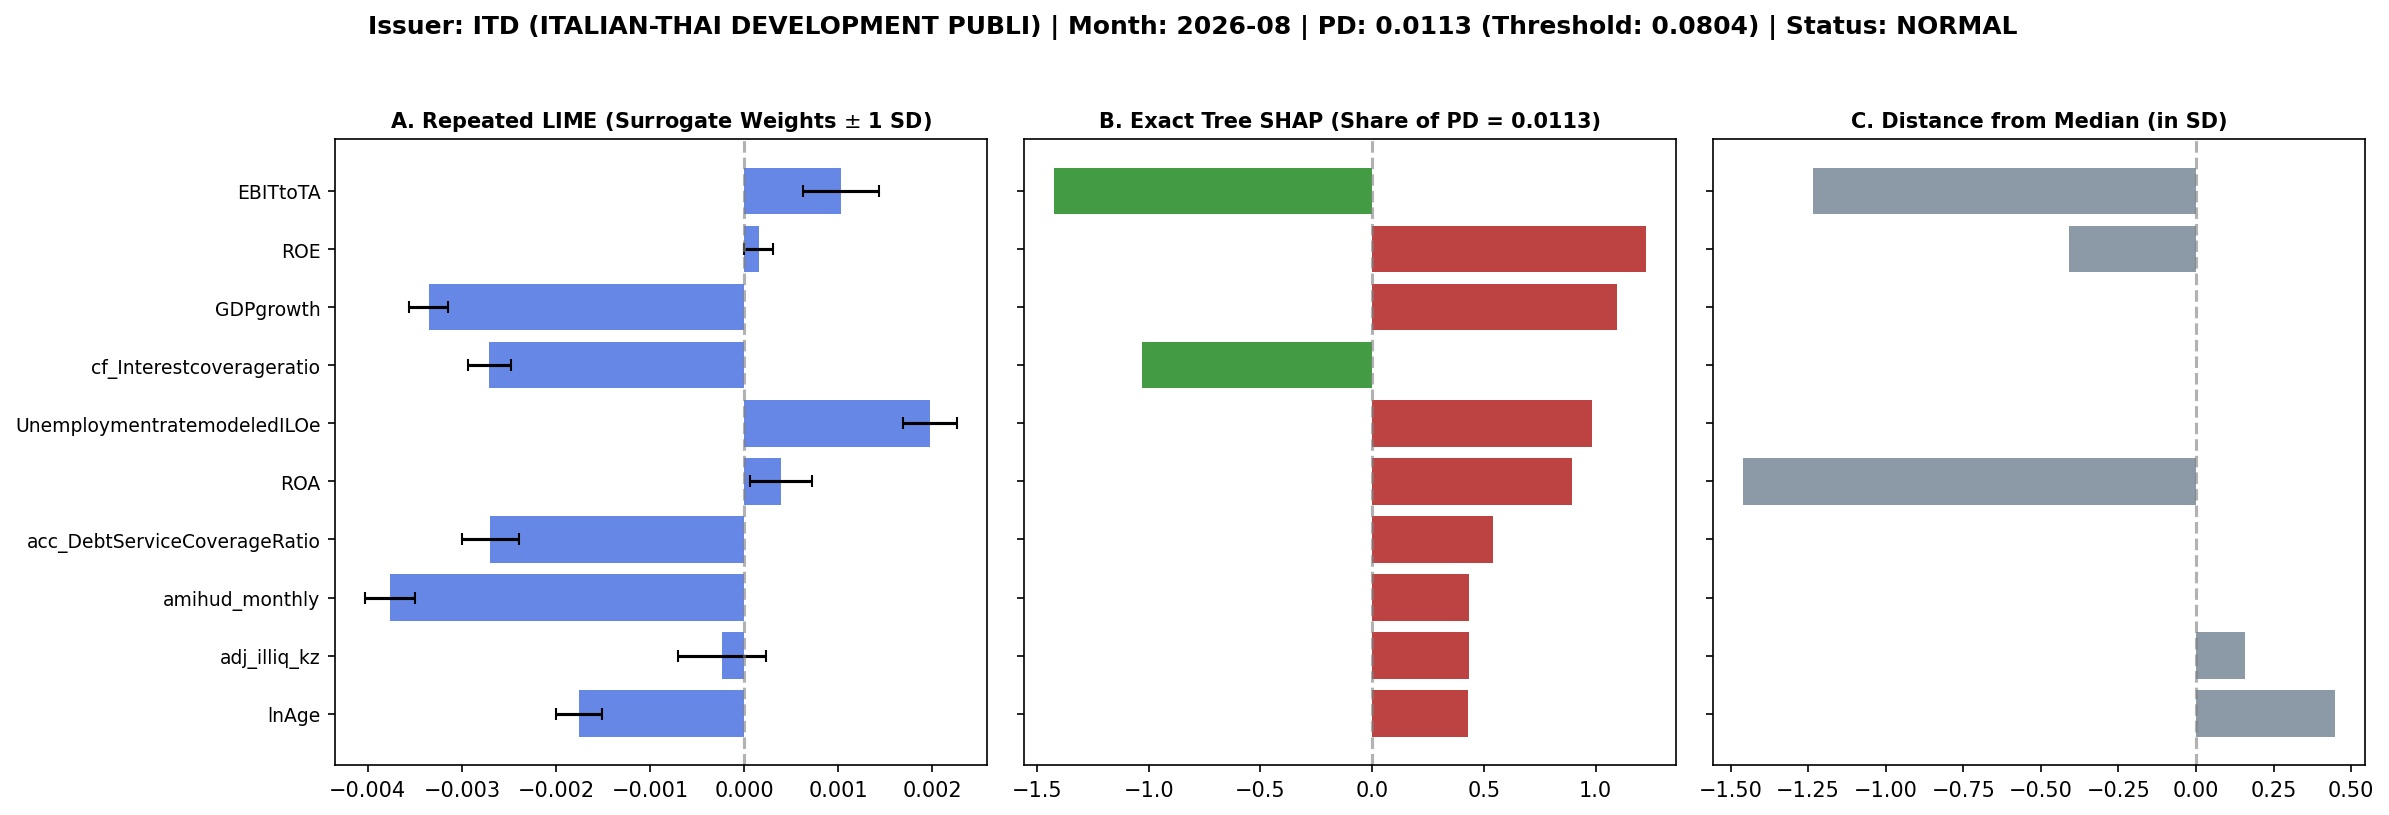
\includegraphics[width=\textwidth]{lime_shap_ITD.jpg}
\caption{ผลของ ITD จาก \texttt{lime33\_adapter\_panel.py -d 2 --segmented -w 12 --issuer ITD}}
\label{fig:itd}
\end{figure}

\textbf{ข้อควรระวังในการอ่านช่อง B ของโปรแกรมหลัก} ค่า SHAP ในช่อง B ของ \path{lime33_adapter_panel.py} คำนวณจากคะแนนดิบของ CatBoost ซึ่งอยู่ในหน่วย log-odds ไม่ใช่หน่วยความน่าจะเป็น แม้ชื่อช่องจะเขียนว่า Share of PD ตัวอย่างของ ITD มีค่า PD 0.0113 แต่แท่ง SHAP ยาวถึง $\pm 1.4$ ซึ่งเป็นไปไม่ได้ถ้าเป็นหน่วย PD คอลัมน์ \path{SHAP_Pct_of_PD} ในไฟล์ Excel จึงไม่ควรอ่านเป็นร้อยละของ PD ทิศทางและลำดับของแท่งยังใช้ได้ ถ้าต้องการค่า SHAP ที่รวมกลับเป็น PD ได้พอดี ให้ใช้ \path{lime_feature33.py} แทน

\textbf{รูปของ \path{lime_feature33.py}} รูปที่~\ref{fig:tpoly} เป็นผลของ TPOLY ช่อง B อยู่ในหน่วยความน่าจะเป็น ค่าฐาน 0.016504 รวมกับผลรวม SHAP $-0.012140$ ได้ PD 0.004364 พอดี ตัวแปรที่มีคำว่า unstable กำกับคือตัวที่ค่า LIME เปลี่ยนเครื่องหมายเมื่อเปลี่ยน seed ไม่ควรนำไปตีความ

\begin{figure}[H]
\centering
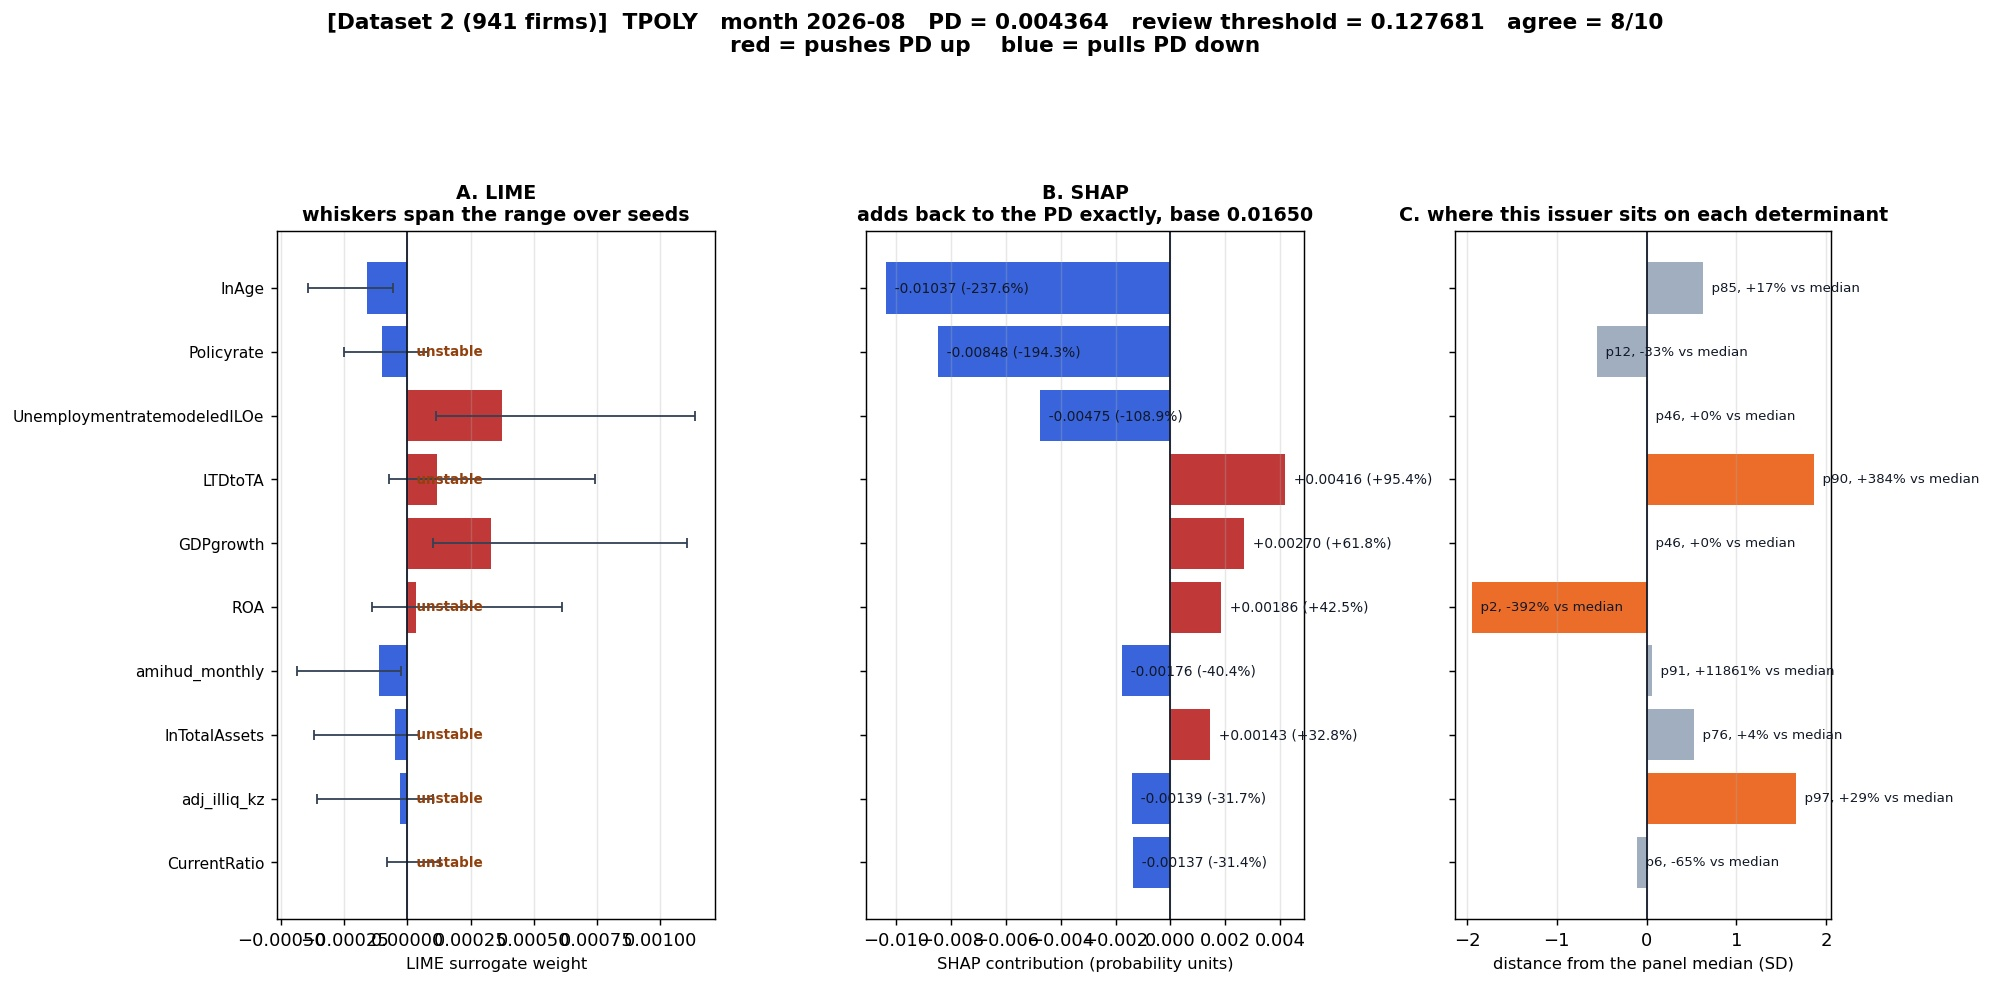
\includegraphics[width=\textwidth]{lime_shap_TPOLY.jpg}
\caption{ผลของ TPOLY จาก \texttt{lime\_feature33.py --issuer TPOLY}}
\label{fig:tpoly}
\end{figure}

\textbf{lead time ของห้าโมเดล (ขั้นที่ 1)} ตาราง~\ref{tab:lead5} ได้ตัวเลขตรงกับรอบที่รันเมื่อ 4 กันยายน 2026 ทุกค่า การเตือนนับเป็นการจับได้เมื่อโมเดลเตือนภายใน 1 ถึง 3 เดือนก่อนเดือนเหตุการณ์ ค่ามัธยฐาน 92 วันจึงเป็นค่าสูงสุดที่เป็นไปได้ของนิยามนี้

\begin{table}[H]
\centering
\small
\caption{ผลของ \texttt{dataset2\_leadtime\_standalone.py} ห้าโมเดล ที่กำลังคน 5\%}
\label{tab:lead5}
\begin{tabular}{@{}lrrrrr@{}}
\toprule
\textbf{โมเดล} & \textbf{AUC} & \textbf{Average precision} & \textbf{จับได้} & \textbf{lead (วัน)} & \textbf{เตือนต่อเนื่อง (วัน)} \\
\midrule
XGBoost & 0.9399 & 0.0150 & 19/31 & 92 & 381.5 \\
CatBoost & 0.9037 & 0.0146 & 20/31 & 92 & 549.0 \\
RandomForest & 0.8846 & 0.0150 & 13/31 & 92 & 397.0 \\
Logistic & 0.8241 & 0.0030 & 9/31 & 92 & 609.0 \\
LightGBM & 0.6599 & 0.0086 & 14/31 & 92 & 486.5 \\
\bottomrule
\end{tabular}
\end{table}

\textbf{LIME ของห้าโมเดล (ขั้นที่ 2)} ตาราง~\ref{tab:mmlime} และรูปที่~\ref{fig:mmlime} คือผลของ \path{dataset2_multimodel_lime.py} ตัวเลขตรงกับรอบ 4 กันยายน 2026 ทุกค่า คอลัมน์สุดท้ายยืนยันว่าโมเดลที่สร้างใหม่ให้ค่า PD ต่างจากขั้นที่ 1 ไม่เกิน $3.4\times10^{-16}$ คือเป็นโมเดลเดียวกัน

\begin{table}[H]
\centering
\small
\caption{ผลของ \texttt{dataset2\_multimodel\_lime.py} (5 seed ละ 750 จุด)}
\label{tab:mmlime}
\begin{tabular}{@{}lrrrr@{}}
\toprule
\textbf{โมเดล} & \textbf{เหตุการณ์ที่อธิบาย} & \textbf{fidelity (R\textsuperscript{2})} & \textbf{ความนิ่งของเครื่องหมาย} & \textbf{ผลต่างของ PD} \\
\midrule
XGBoost & 19/31 & 0.019 & 1.0 & $1.1\times10^{-16}$ \\
CatBoost & 20/31 & 0.000 & 0.8 & $1.1\times10^{-16}$ \\
RandomForest & 13/31 & 0.013 & 1.0 & $3.3\times10^{-16}$ \\
Logistic & 9/31 & 0.555 & 1.0 & $1.1\times10^{-16}$ \\
LightGBM & 14/31 & 0.070 & 1.0 & $1.1\times10^{-16}$ \\
\bottomrule
\end{tabular}
\end{table}

\begin{figure}[H]
\centering
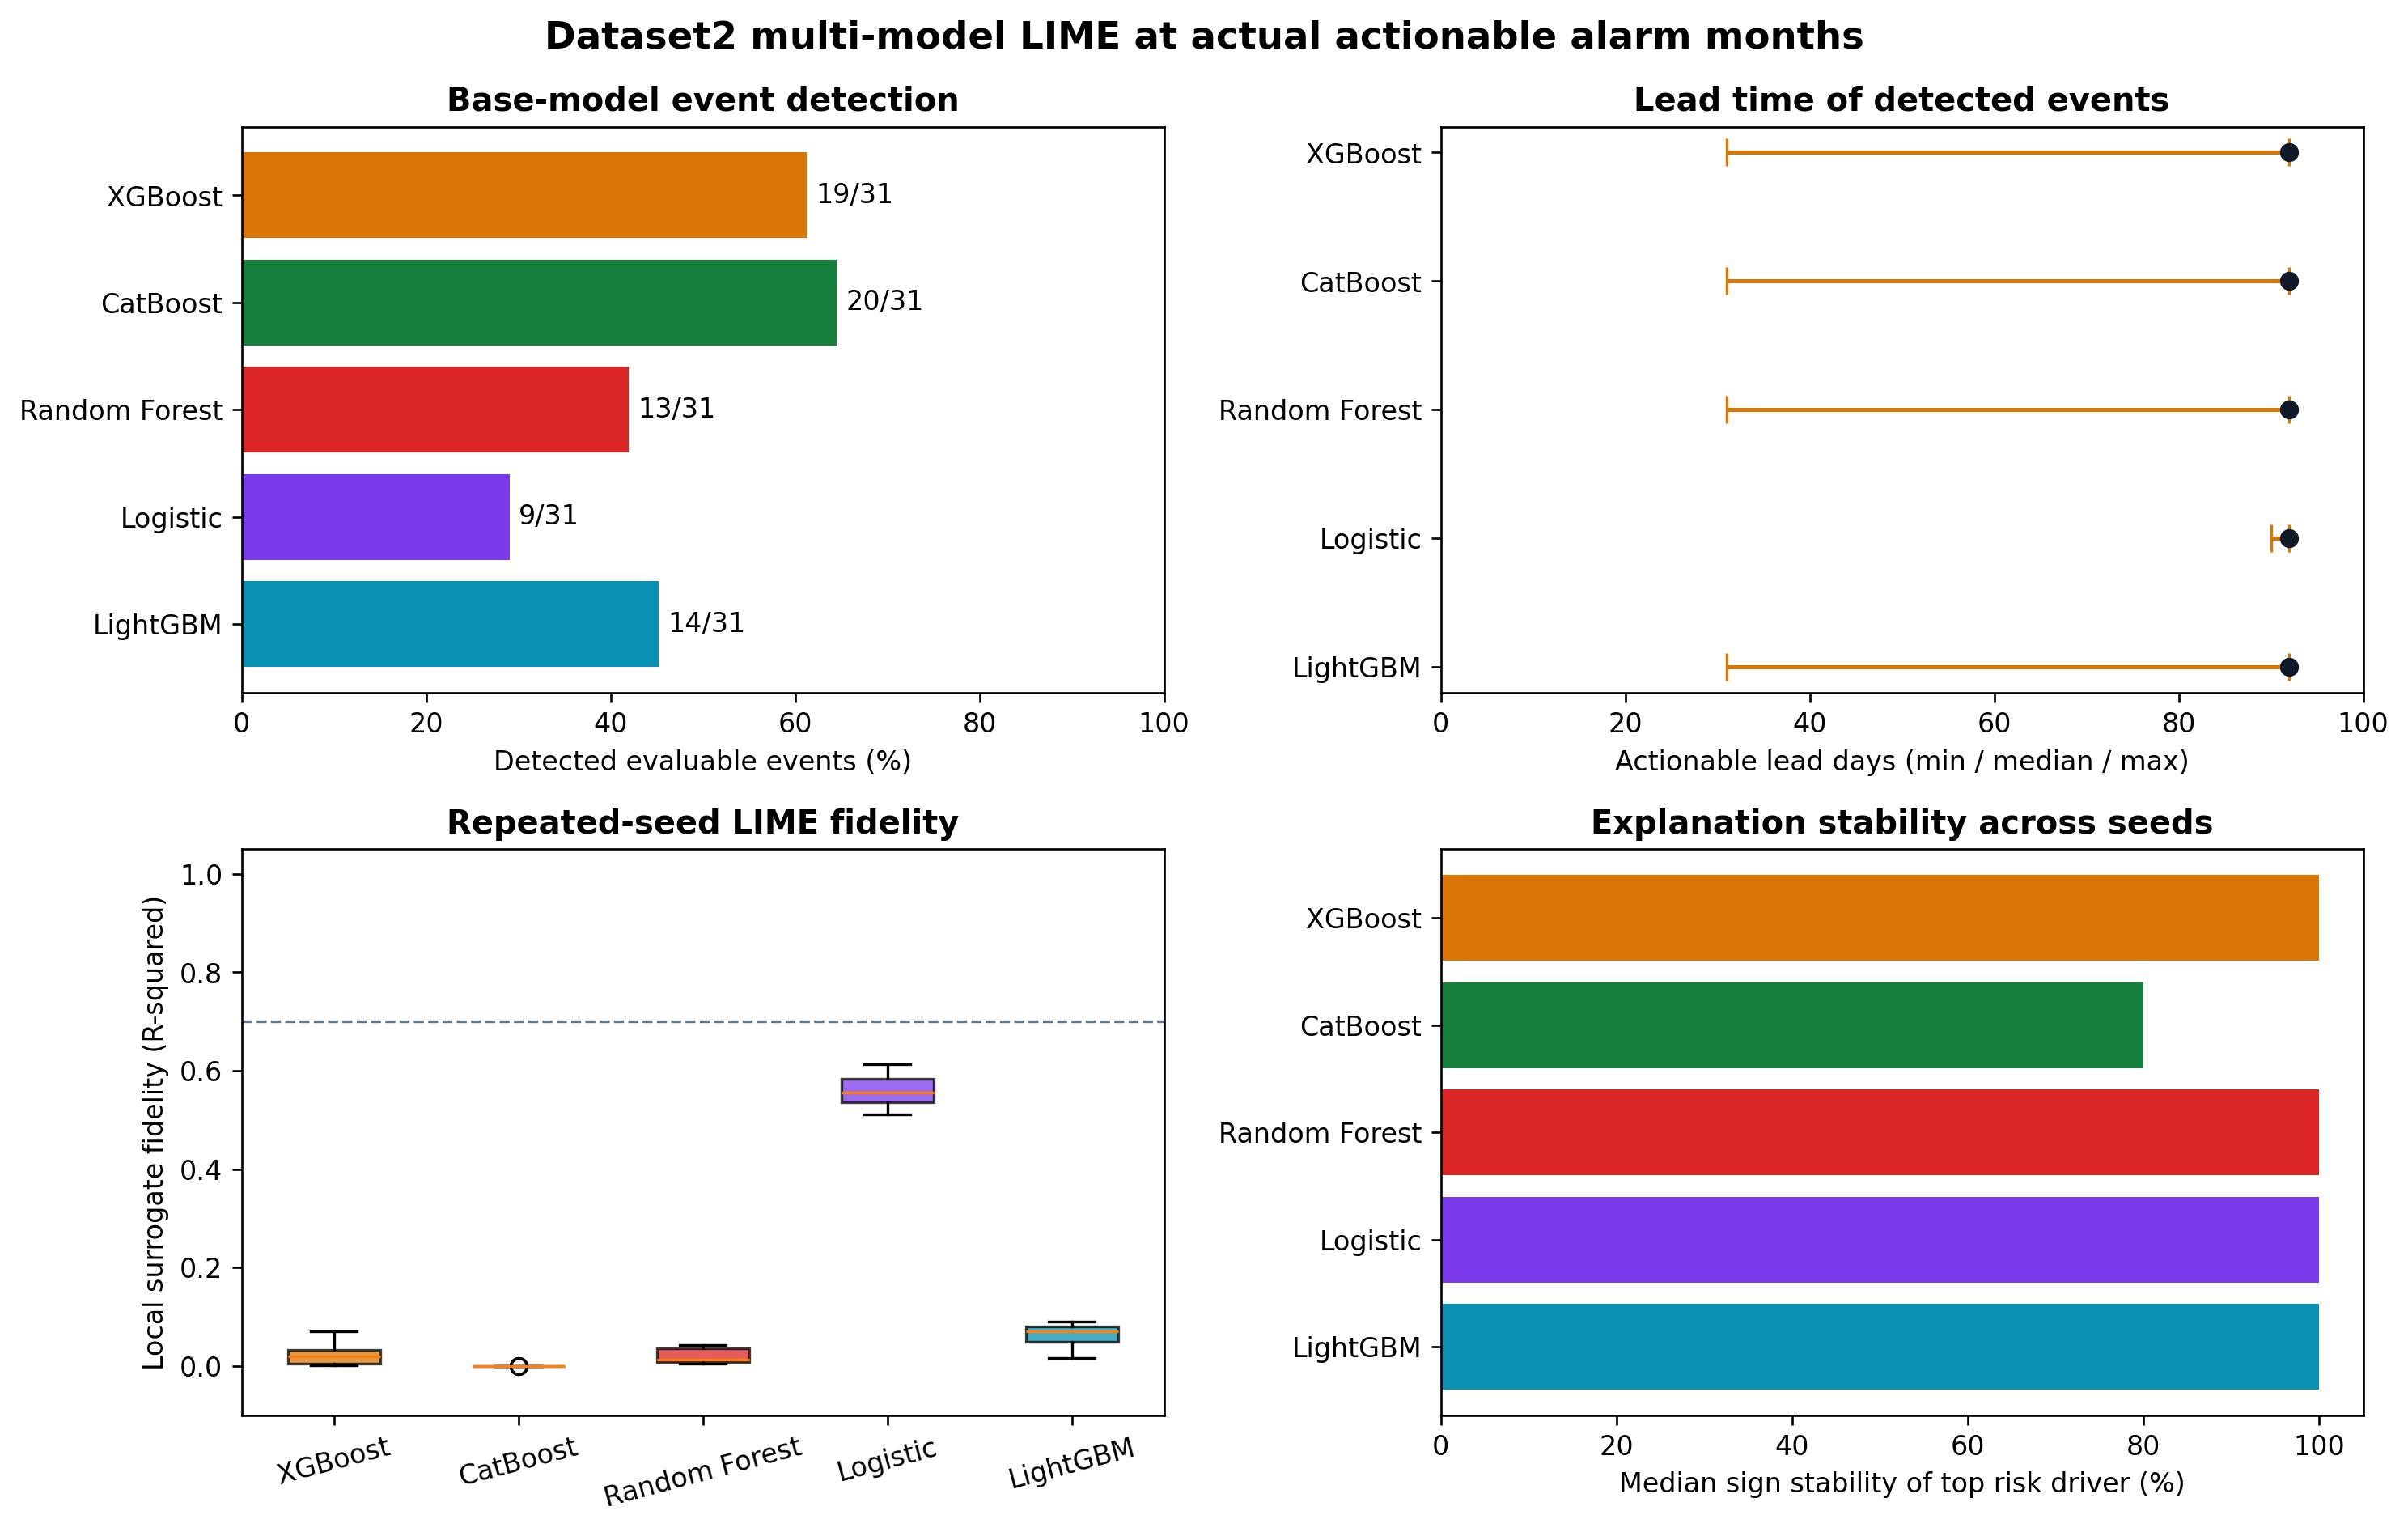
\includegraphics[width=\textwidth]{multimodel_lime_summary.jpg}
\caption{สรุป LIME ของห้าโมเดล ณ เดือนที่เตือนจริง}
\label{fig:mmlime}
\end{figure}

\textbf{อ่านค่า fidelity อย่างไร} fidelity คือ R\textsuperscript{2} ของเส้นตรงที่ LIME ฟิตรอบจุดนั้น เทียบกับค่าที่โมเดลจริงให้ ค่ามัธยฐานของโมเดลกลุ่มต้นไม้ต่ำมาก อยู่ระหว่าง 0.000 ถึง 0.070 มีเพียง Logistic ที่ได้ 0.555 เพราะโมเดลเองเป็นเส้นตรงอยู่แล้ว แปลว่าสำหรับโมเดลกลุ่มต้นไม้ เส้นตรงของ LIME อธิบายพฤติกรรมเฉพาะที่ของโมเดลได้น้อย น้ำหนัก LIME จึงบอกทิศทางคร่าว ๆ ได้ แต่ไม่ควรอ่านขนาดของน้ำหนักเป็นตัวเลขที่แม่น ในกรณีนี้ควรดูค่า SHAP ประกอบ

\textbf{วิธี A, B, C บน Dataset2} ตาราง~\ref{tab:abc} คือผลของ \path{evaluate_methods_abc.py} ส่วนของชุดที่ 2 วิธี A คือ PD เหนือเส้น วิธี B คือบริษัทที่ขยับตัวแปรเดียวไม่เกิน 1 SD ก็ข้ามเส้น วิธี C คือกำไรสะสมและเงินสดอยู่ใน decile ล่างสุดทั้งคู่

\begin{table}[H]
\centering
\small
\caption{วิธี A, B, C บน Dataset2 ที่กำลังคน 5\%}
\label{tab:abc}
\begin{tabular}{@{}lrrrr@{}}
\toprule
\textbf{วิธี} & \textbf{เตือน (ราย)} & \textbf{จับได้} & \textbf{Recall} & \textbf{Precision} \\
\midrule
A ระดับ PD & 48 & 8/31 & 25.8\% & 16.7\% \\
B ความเปราะบาง & 21 & 3/31 & 9.7\% & 14.3\% \\
C งบแย่ที่ถูกบัง & 39 & 5/31 & 16.1\% & 12.8\% \\
A + C & 87 & 13/31 & 41.9\% & 14.9\% \\
A + B + C & 106 & 15/31 & 48.4\% & 14.2\% \\
\bottomrule
\end{tabular}
\end{table}

บนชุดที่ 1 วิธีเดียวกันจับได้ครบ 8 จาก 8 ราย แต่เกณฑ์ทุกชั้นเลือกจากเหตุการณ์ 8 รายชุดเดียวกับที่ใช้วัดผล ตัวเลขนั้นจึงเข้าข้างตัวเอง บน Dataset2 ซึ่งมีเหตุการณ์ใหม่ 31 ราย วิธีเดียวกันจับได้ 15 ราย เป็นตัวเลขที่สะท้อนความสามารถจริงมากกว่า

% ====================================================================
\section*{5. คลังที่สอง leadning\_time: วัด lead time}

\subsection*{5.1 หน้าที่ของคลัง}

คลังนี้ตอบว่าระบบเตือนก่อนเหตุการณ์จริงได้กี่เดือน และจับบริษัทที่เกิดเหตุการณ์ได้กี่ราย มีสองโปรแกรมที่นิยาม lead time ต่างกัน จึงต้องอ่านผลแยกกัน

\begin{itemize}[leftmargin=1.6em, itemsep=2pt]
\item \path{dynamic_lead_time.py} ใช้หน้าต่าง T$-$12 ถึง T$+$3 รอบเดือนเหตุการณ์ T และรายงานสามแบบ คือ broad (T$-$12 ถึง T$+$3), early-only (T$-$12 ถึง T$-$1) และ strict (T$-$3 ถึง T$-$1) lead time คือเดือนเหตุการณ์ลบเดือนที่เตือนครั้งแรก มีทั้งแบบแบ่ง fold ตามบริษัท และแบบฝึกด้วยอดีตแล้วทดสอบปีถัดไป (time-forward)
\item \path{dataset2_leadtime_standalone.py} นับเป็นการจับได้เฉพาะเมื่อเตือนภายใน 1 ถึง 3 เดือนปฏิทินก่อนเหตุการณ์ lead time จึงไม่เกิน 92 วัน และวัดความยาวของการเตือนต่อเนื่องแยกไว้ รันได้เก้าโมเดลด้วยการแบ่ง fold เดียวกัน
\end{itemize}

\subsection*{5.2 โครงสร้างโปรแกรม}

\begin{table}[H]
\centering
\small
\caption{ไฟล์ในคลัง leadning\_time}
\label{tab:lead-files}
\begin{tabular}{@{}p{5.4cm}p{8.8cm}@{}}
\toprule
\textbf{ไฟล์} & \textbf{หน้าที่} \\
\midrule
\path{dynamic_lead_time.py} & lead time แบบหน้าต่าง T$-$12 ถึง T$+$3 ทั้งแบบแบ่งตามบริษัทและแบบ time-forward \\
\path{dataset2_leadtime_standalone.py} & lead time 1 ถึง 3 เดือนของเก้าโมเดล (ไฟล์เดียวกับใน iBond\_LIME) \\
\path{lime_credit.db.zip} & Dataset2 แบบบีบอัด คลายเองในการรันครั้งแรก \\
\path{run_dynamic_lead_time.bat} & ดับเบิลคลิกเพื่อรัน \path{dynamic_lead_time.py} บน Windows \\
\path{requirements*.txt} & รายการแพ็กเกจ สามระดับ พื้นฐาน, CatBoost และครบทั้งคลัง \\
\path{tests/test_core.py} & ทดสอบฟังก์ชันคำนวณ lead time \\
\path{results/} & ผลอ้างอิง Excel, SQLite และ CSV \\
\path{docs/} & คู่มือ LaTeX ภาษาไทยเดิมของโปรแกรมแรก และคู่มือฉบับนี้ \\
\bottomrule
\end{tabular}
\end{table}

\subsection*{5.3 วิธีรัน \texttt{dynamic\_lead\_time.py}}

\begin{Cmd}
python dynamic_lead_time.py
python dynamic_lead_time.py --model catboost
python dynamic_lead_time.py --model numpy
python dynamic_lead_time.py --skip-time-forward
python dynamic_lead_time.py --db ..\iBond_LIME\lime_credit.db
python -m unittest discover -s tests -v
\end{Cmd}

\begin{table}[H]
\centering
\small
\caption{ตัวเลือกหลักของ \texttt{dynamic\_lead\_time.py}}
\label{tab:dlt-opts}
\begin{tabular}{@{}p{3.8cm}p{2.2cm}p{8.2cm}@{}}
\toprule
\textbf{ตัวเลือก} & \textbf{ค่าเริ่มต้น} & \textbf{ความหมาย} \\
\midrule
\path{--model} & auto & auto ใช้ CatBoost ถ้าติดตั้งไว้ ถ้าไม่มีใช้ logistic ที่เขียนด้วย numpy \\
\path{--feature-set} & report30 & report30 คือตัวแปร 30 ตัวของรายงาน correct33 คือ 33 คอลัมน์ \\
\path{--workload} & 0.05 & กำลังคนที่ใช้ตั้งเส้นเตือนภัย \\
\path{--window-before}, \path{--window-after} & 12, 3 & ขอบของหน้าต่างรอบเดือนเหตุการณ์ \\
\path{--skip-time-forward} & -- & ข้ามการทดสอบแบบ time-forward เพื่อลดเวลา \\
\path{--db}, \path{--table} & ค้นหาเอง & ระบุฐานข้อมูลและตารางเอง \\
\path{--no-excel}, \path{--no-sqlite}, \path{--no-csv} & -- & ไม่เขียนผลแบบนั้น \\
\bottomrule
\end{tabular}
\end{table}

โปรแกรมค้นหาฐานข้อมูลเองตามลำดับ คือ path ที่ระบุด้วย \path{--db} โฟลเดอร์ที่รันอยู่ โฟลเดอร์ของโปรแกรม โฟลเดอร์แม่ และโฟลเดอร์ย่อย \path{data/} ชื่อที่ค้นคือ \path{cmdf_credit.db}, \path{lime_credit.db} และ \path{bond_financials.db} ถ้าไม่พบเลยจะคลาย \path{lime_credit.db.zip} ที่แนบมา ผลเขียนลง \path{results/dynamic_lead_time_results.xlsx}, \path{results/dynamic_lead_time_results.db} และ \path{results/csv/}

\subsection*{5.4 วิธีรัน \texttt{dataset2\_leadtime\_standalone.py}}

\begin{Cmd}
python dataset2_leadtime_standalone.py --version
python dataset2_leadtime_standalone.py self-test
python dataset2_leadtime_standalone.py inspect
python dataset2_leadtime_standalone.py run
python dataset2_leadtime_standalone.py run --models xgboost catboost --workload 0.10
python dataset2_leadtime_standalone.py build-db
\end{Cmd}

\begin{table}[H]
\centering
\small
\caption{คำสั่งย่อยของ \texttt{dataset2\_leadtime\_standalone.py}}
\label{tab:std-cmds}
\begin{tabular}{@{}p{2.6cm}p{11.6cm}@{}}
\toprule
\textbf{คำสั่งย่อย} & \textbf{ทำอะไร} \\
\midrule
\path{self-test} & ตรวจสูตร lead time, precision-recall ตาม workload และ probit ด้วยข้อมูลสมมติ ไม่ต้องใช้ฐานข้อมูล \\
\path{inspect} & นับแถว บริษัท เดือน เหตุการณ์ และตรวจแถวซ้ำของตาราง Dataset2 \\
\path{run} & ฝึกโมเดลด้วยการแบ่ง fold ตามบริษัท 5 fold แล้ววัด lead time ค่าเริ่มต้นรันครบเก้าโมเดล ระบุบางตัวด้วย \path{--models} ชื่อที่ใช้ได้คือ xgboost, catboost, lightgbm, random\_forest, logistic, probit, hist\_gradient\_boosting, gradient\_boosting, extra\_trees \\
\path{build-db} & คัดตาราง Dataset2 และตาราง iBond ดิบที่มีอยู่ ไปเป็นฐานข้อมูลชุดใหม่ใน \path{standalone_dataset2/} ฐานข้อมูลต้นทางไม่ถูกแก้ \\
\path{update-ibond} & สร้างฐานข้อมูลชุดใหม่ที่ปรับเหตุการณ์ผิดนัดจาก iBond ต้องระบุ \path{--base-db} และเลือกหนึ่งทาง คือ \path{--from-db} อ่านตาราง iBond ที่ดาวน์โหลดไว้แล้ว หรือ \path{--download} ซึ่งต้องมี \path{download_bond.py} ของ ibond\_EWS และรหัสผ่าน iBond ของผู้ใช้เอง \\
\bottomrule
\end{tabular}
\end{table}

ผลของ \path{run} อยู่ในโฟลเดอร์ \path{standalone_leadtime_runs/standalone_<date>_<time>_<id>/} มีตารางสรุปโมเดล lead time ของทุกเหตุการณ์ precision-recall ที่กำลังคน 1\% ถึง 10\% ค่า PD แบบ out-of-fold ทุกแถว ฐานข้อมูล SQLite และรูปสามรูป

\subsection*{5.5 ผลการรันบน Dataset2}

\textbf{\path{dynamic_lead_time.py} ให้ผลต่างกันตาม backend} ผลที่แนบในคลังเดิมรันในเครื่องที่ไม่มี CatBoost และไม่มี scikit-learn จึงใช้ logistic แบบ numpy กับการแบ่ง fold ที่เขียนเอง รอบนี้รันครบทั้งสามแบบบนเครื่องเดียวกัน ตาราง~\ref{tab:dlt} แสดงว่าผลขึ้นกับแพ็กเกจที่ติดตั้งอย่างมาก ผู้ใช้ต้องดูบรรทัด Model backend ที่โปรแกรมพิมพ์ทุกครั้งก่อนอ่านตัวเลข

\begin{table}[H]
\centering
\small
\caption{ผลของ \texttt{dynamic\_lead\_time.py} บน Dataset2 แยกตาม backend}
\label{tab:dlt}
\begin{tabular}{@{}lrrr@{}}
\toprule
\textbf{รายการ} & \textbf{CatBoost} & \textbf{numpy + sklearn fold} & \textbf{numpy + fold เขียนเอง} \\
\midrule
แบ่งตามบริษัท broad & 24/31 = 77.4\% & 14/31 = 45.2\% & 13/31 = 41.9\% \\
แบ่งตามบริษัท early-only & 22/31 = 71.0\% & 11/31 = 35.5\% & 10/31 = 32.3\% \\
แบ่งตามบริษัท strict 1--3 เดือน & 21/31 = 67.7\% & 11/31 = 35.5\% & 10/31 = 32.3\% \\
time-forward broad & 14/26 = 53.8\% & 8/26 = 30.8\% & 8/26 = 30.8\% \\
time-forward early-only & 11/26 = 42.3\% & 6/26 = 23.1\% & 6/26 = 23.1\% \\
time-forward strict 1--3 เดือน & 9/26 = 34.6\% & 6/26 = 23.1\% & 6/26 = 23.1\% \\
คิวเตือน 12 เดือนล่าสุด (ราย) & 256 & 151 & -- \\
\bottomrule
\end{tabular}
\end{table}

\noindent คอลัมน์สุดท้ายคัดจากผลเดิมที่แนบในคลังก่อนรอบนี้ time-forward ประเมินได้ 26 ราย เพราะอีก 5 รายเกิดเหตุการณ์ในปี 2020--2021 ก่อนหน้านั้นยังไม่มีบริษัทที่เกิดเหตุการณ์ให้โมเดลเรียน ผลที่แนบในคลังรอบนี้เปลี่ยนเป็นผลของ CatBoost เพราะเป็นสิ่งที่ผู้ใช้จะได้เมื่อติดตั้งตาม \path{requirements-catboost.txt}

ผลแบบ early-only ของ CatBoost ได้ 22/31 เท่ากับตัวเลข 71.0\% ที่รายงาน LIME เคยอ้าง แต่โปรแกรมเทียบตัวเลขนั้นกับแบบ broad ซึ่งได้ 24/31 สถานะที่พิมพ์ออกมาจึงเป็น NO\_MATCH ผลแบบแบ่งตามบริษัทยังมีความเสี่ยงที่โมเดลได้เห็นข้อมูลปีหลังตอนทำนายปีก่อน ผลที่ใกล้การใช้งานจริงกว่าคือแบบ time-forward

\textbf{เก้าโมเดลของ \path{dataset2_leadtime_standalone.py}} ตาราง~\ref{tab:nine} คือผลของ \path{python dataset2_leadtime_standalone.py run} ซึ่งรันครบเก้าโมเดลใน 677 วินาที ในจำนวนนี้ GradientBoosting ใช้ 471 วินาที ห้าโมเดลแรกที่ตรงกับตาราง~\ref{tab:lead5} ได้ตัวเลขเท่ากันทุกค่า เพราะใช้การแบ่ง fold ชุดเดียวกัน

\begin{table}[H]
\centering
\small
\caption{ผลของ \texttt{dataset2\_leadtime\_standalone.py run} เก้าโมเดล ที่กำลังคน 5\%}
\label{tab:nine}
\begin{tabular}{@{}lrrrrr@{}}
\toprule
\textbf{โมเดล} & \textbf{AUC} & \textbf{Average precision} & \textbf{จับได้} & \textbf{เตือนต่อเนื่อง (วัน)} & \textbf{วินาที} \\
\midrule
XGBoost & 0.9399 & 0.0150 & 19/31 & 381.5 & 7 \\
CatBoost & 0.9037 & 0.0146 & 20/31 & 549.0 & 26 \\
LightGBM & 0.6599 & 0.0086 & 14/31 & 486.5 & 9 \\
RandomForest & 0.8846 & 0.0150 & 13/31 & 397.0 & 52 \\
Logistic & 0.8241 & 0.0030 & 9/31 & 609.0 & 6 \\
Probit & 0.8350 & 0.0033 & 12/31 & 306.0 & 16 \\
HistGradientBoosting & 0.8777 & 0.0259 & 18/31 & 397.0 & 8 \\
GradientBoosting & 0.9331 & 0.0154 & 20/31 & 411.0 & 471 \\
ExtraTrees & 0.8875 & 0.0122 & 20/31 & 670.0 & 46 \\
\bottomrule
\end{tabular}
\end{table}

\textbf{อ่านตารางนี้อย่างไร} AUC สูงสุดคือ XGBoost 0.9399 average precision สูงสุดคือ HistGradientBoosting 0.0259 และจับได้มากที่สุด 20 จาก 31 ราย มีสามโมเดล คือ CatBoost, GradientBoosting และ ExtraTrees ค่า average precision ดูต่ำเพราะเดือนที่เกิดเหตุการณ์มีเพียงร้อยละ 0.066 ของข้อมูล ค่าที่ได้จากการเดาสุ่มจึงเท่ากับ 0.00066 XGBoost ได้ 0.0150 สูงกว่าการเดาสุ่มราว 23 เท่า ไฟล์ผลยังมีคอลัมน์ \path{pr_auc_trapezoid_oof} ซึ่งคำนวณด้วยวิธีสี่เหลี่ยมคางหมูและเชื่อไม่ได้เมื่อเส้น precision-recall ไม่เรียบ เช่น LightGBM ได้ 0.0954 ทั้งที่ average precision เพียง 0.0086 ให้อ่านคอลัมน์ \path{average_precision_oof} แทน

รูปที่~\ref{fig:leadmatrix} แสดงผลรายบริษัทของทุกโมเดล ช่องสีเขียวคือเตือนภายใน 1 ถึง 3 เดือนก่อนเหตุการณ์ พร้อมจำนวนวัน ช่องสีแดงคือไม่มีการเตือนในช่วงนั้น ช่องสีเทาคือไม่มีข้อมูลก่อนเหตุการณ์ ACAP, EA, JTS และ TPCH ไม่มีโมเดลใดจับได้ ส่วน WSOL ไม่มีข้อมูลก่อนเดือนเหตุการณ์จึงประเมินไม่ได้

\begin{figure}[H]
\centering
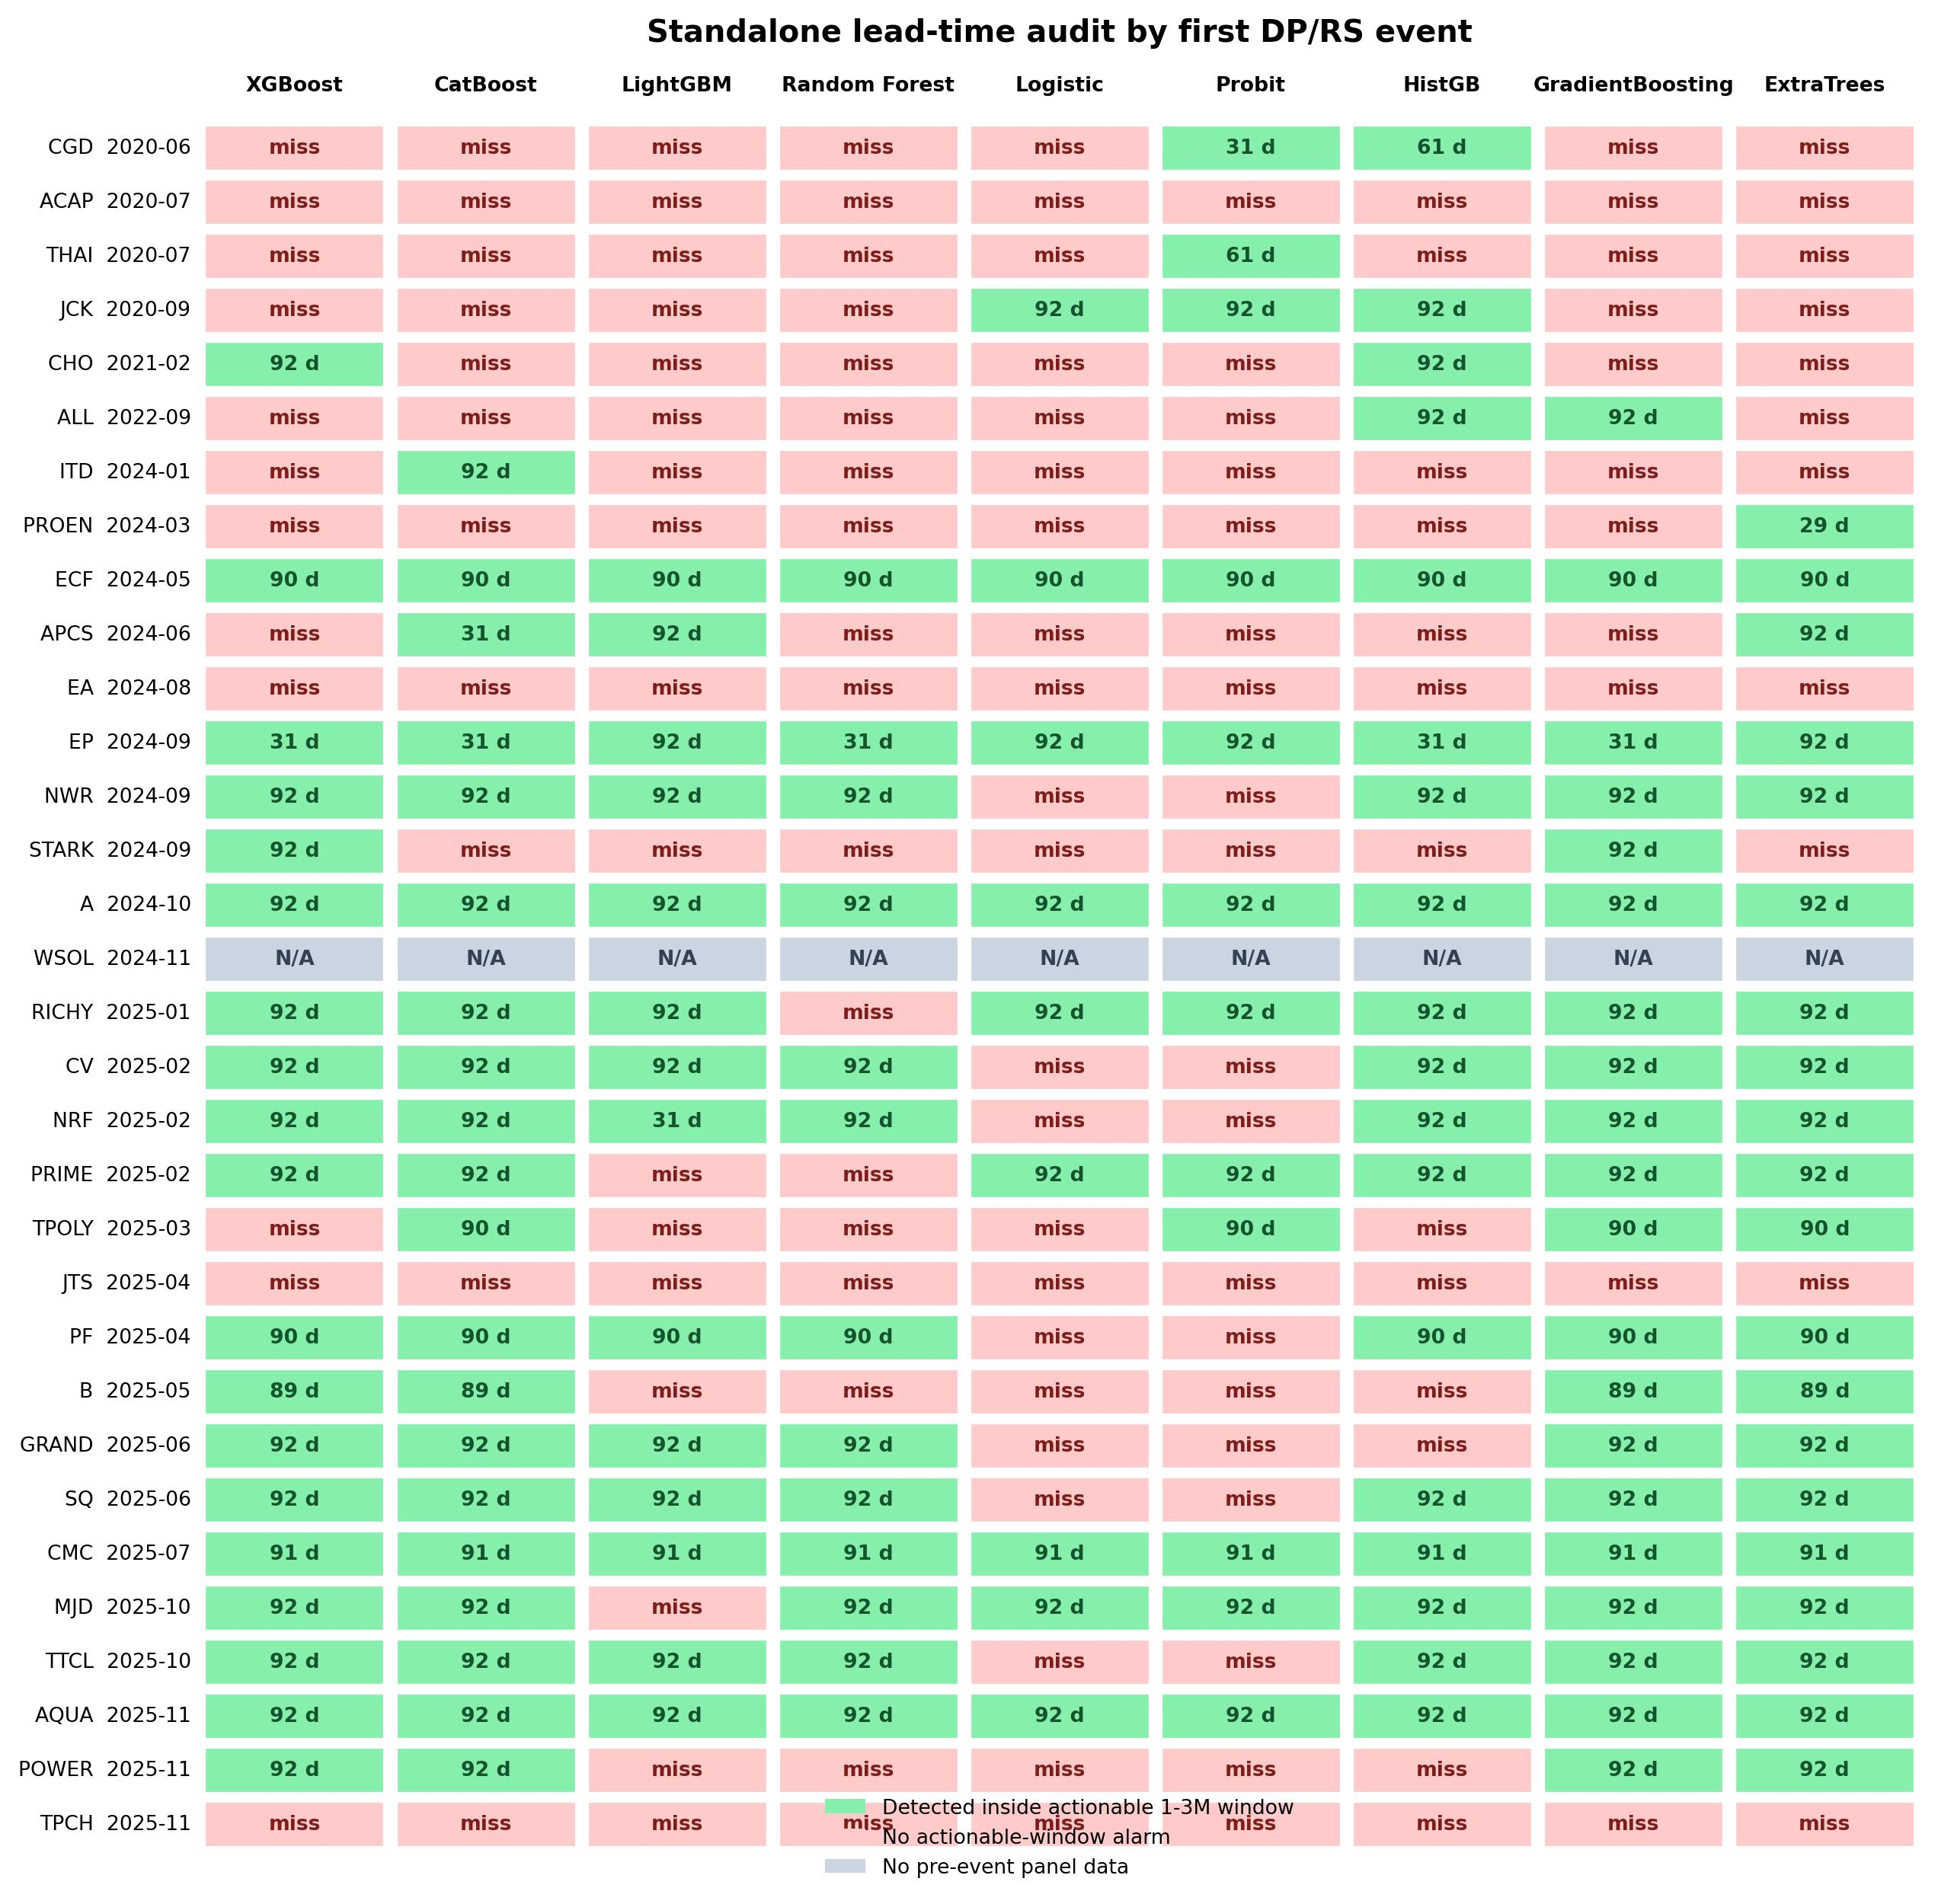
\includegraphics[width=0.93\textwidth]{standalone_lead_matrix.jpg}
\caption{ผลรายบริษัทของเก้าโมเดล จาก \texttt{standalone\_lead\_matrix.jpg}}
\label{fig:leadmatrix}
\end{figure}

รูปที่~\ref{fig:prcurve} แสดง precision และ recall เมื่อเพิ่มกำลังคนจาก 1\% ถึง 10\% ของบริษัท-เดือน เมื่อตรวจมากขึ้น recall เพิ่มขึ้นแต่ precision ลดลง โมเดลกลุ่มต้นไม้ทุกตัวยกเว้น LightGBM อยู่เหนือ Logistic และ Probit ทุกระดับกำลังคน ส่วน LightGBM ใกล้เคียง Probit เมื่อกำลังคนตั้งแต่ 6\% ขึ้นไป

\begin{figure}[H]
\centering
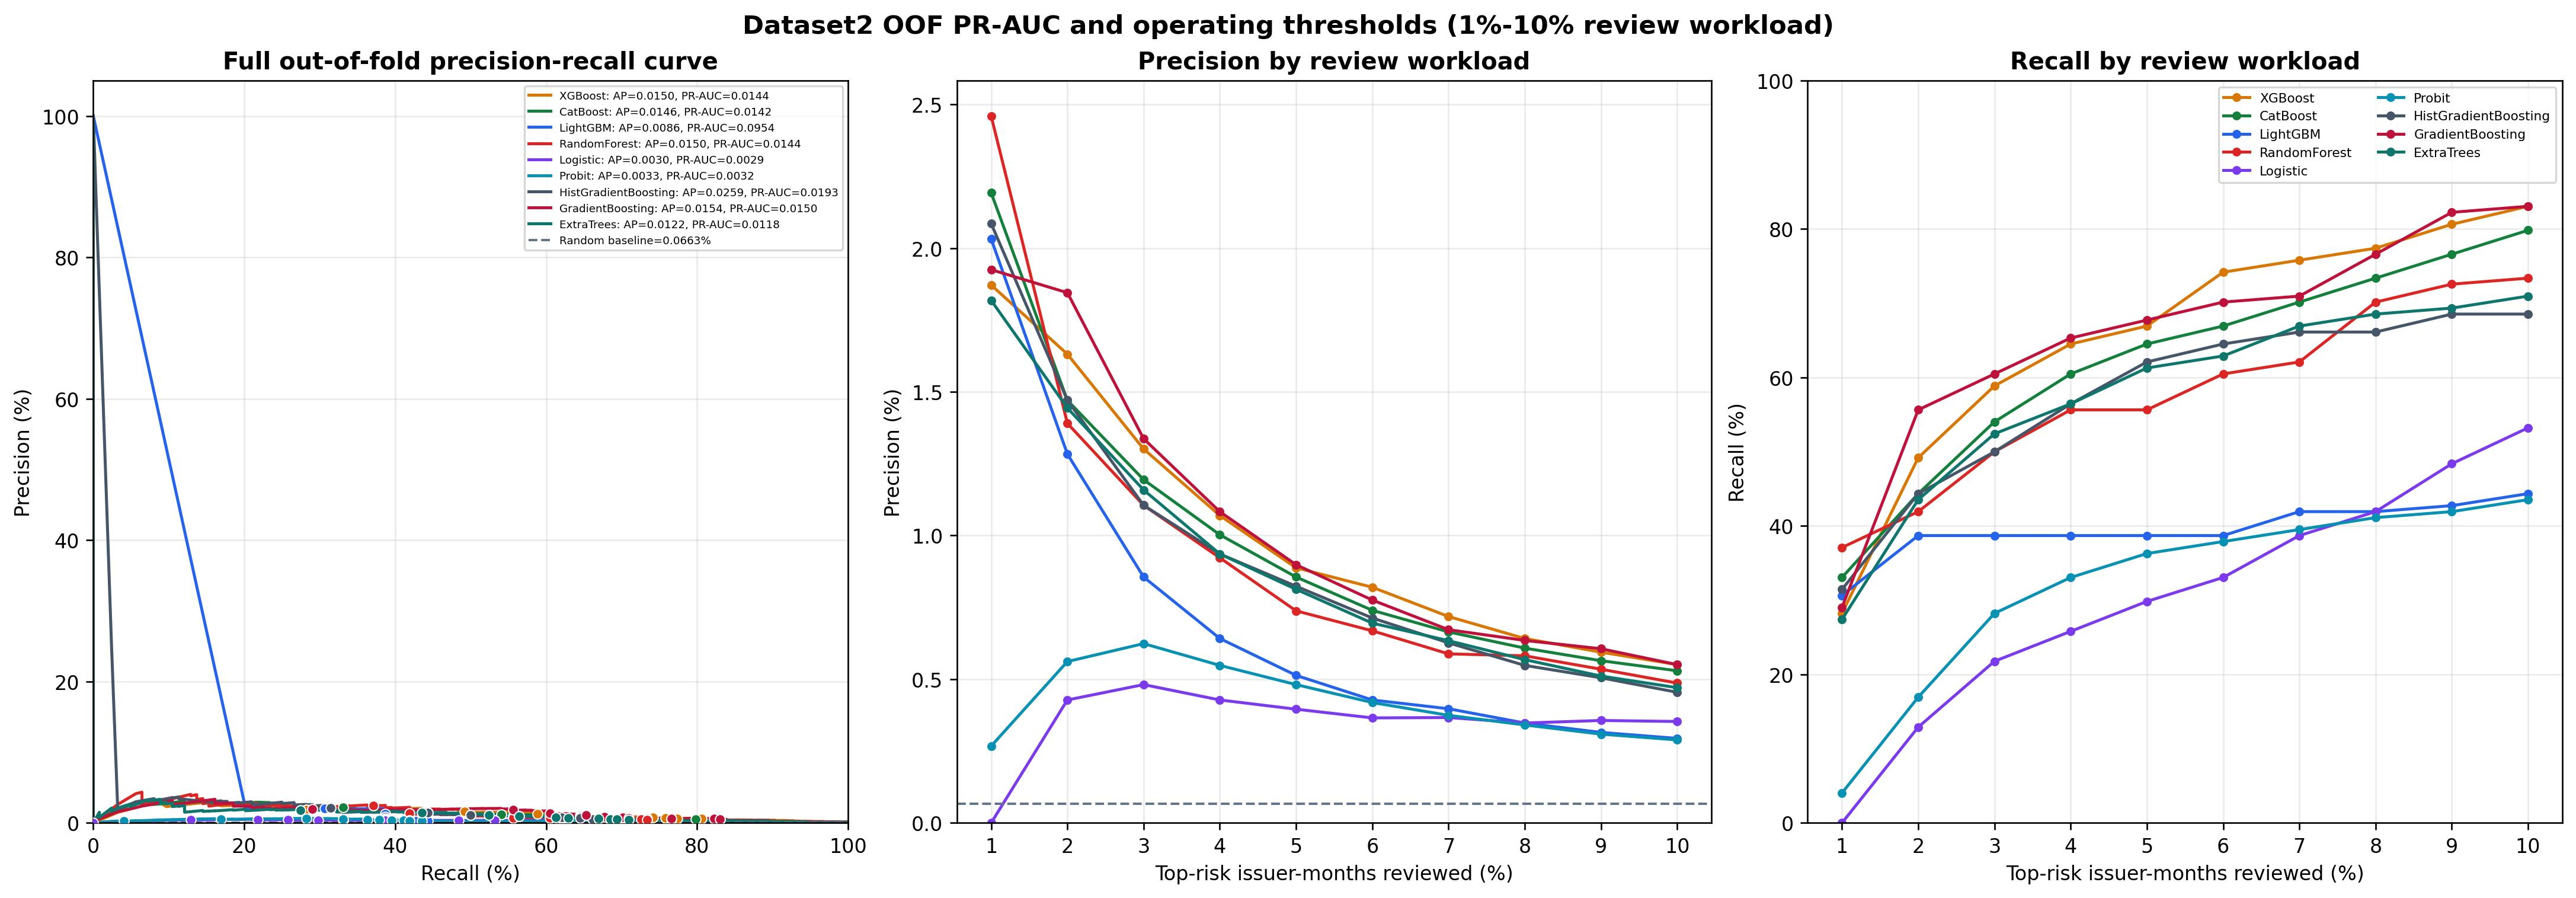
\includegraphics[width=\textwidth]{precision_recall_curve_1_10pct.jpg}
\caption{precision และ recall ตามกำลังคน 1\% ถึง 10\% จาก \texttt{precision\_recall\_curve\_1\_10pct.jpg}}
\label{fig:prcurve}
\end{figure}

ผลอ้างอิงของรอบนี้แนบไว้ในคลังที่ \path{results/standalone_reference/} ได้แก่ตารางสรุปโมเดล lead time ของทุกเหตุการณ์ precision-recall ตามกำลังคน คะแนนเดือนล่าสุด และรูปสามรูป ไม่ได้แนบค่า PD ทุกแถวและฐานข้อมูลผลเพราะมีขนาดรวมราว 35 MB รันใหม่ได้ด้วยคำสั่งเดียว

% ====================================================================
\section*{6. คลังที่สาม ibond\_EWS: ระบบเตือนภัยและหน้าจอโปรแกรม}

\subsection*{6.1 หน้าที่ของคลัง}

คลังนี้เป็นระบบเตือนภัยเต็มรูปแบบ ตอบสองคำถามหลักรายบริษัท คือตอนนี้อยู่ห่างจากเส้นเตือนภัยเท่าไร และตัวแปรใดต้องขยับไปเท่าไรจึงจะข้ามเส้น มีหน้าจอโปรแกรมที่เขียนด้วย Flet โปรแกรมคำนวณ PD หลายแบบ การ shock ตัวแปร การดึงข้อมูลจาก iBond และการแจ้งเตือนทางอีเมล รอบนี้เพิ่มโฟลเดอร์ \path{dataset2/} ซึ่งเป็นระบบเดียวกันที่ทำงานบน Dataset2

\subsection*{6.2 โครงสร้างโปรแกรม}

\begin{table}[H]
\centering
\small
\caption{โฟลเดอร์ในคลัง ibond\_EWS}
\label{tab:ews-folders}
\begin{tabular}{@{}p{3.6cm}rp{9.4cm}@{}}
\toprule
\textbf{โฟลเดอร์} & \textbf{ไฟล์} & \textbf{เนื้อหา} \\
\midrule
ราก & 2 & \path{run.py} ตัวเรียกโปรแกรม และ \path{thaibma_paths.py} ตัวหาฐานข้อมูล \\
\path{app/} & 7 & หน้าจอโปรแกรม \path{app.py} การเฝ้าระวัง อีเมล และ \path{pd11_panel.py} \\
\path{app/legacy/} & 7 & หน้าจอรุ่นเก่า เก็บไว้อ้างอิง \\
\path{ews/} & 16 & แกนของระบบ PD เส้นเตือนภัย โมเมนตัม การ shock รายบริษัท และ LIME \\
\path{models/} & 17 & โมเดลกลุ่มต้นไม้ เส้นอัตราผลตอบแทน และ Koopman \\
\path{analysis/} & 15 & การ shock ทีละคู่และทีละสาม PCA และความสำคัญของตัวแปร \\
\path{reanalysis/} & 3 & การประเมินรอบใหม่ตามข้อท้วงติงของผู้ประเมินบทความ \\
\path{data/} & 22 & ดึงข้อมูล iBond สร้างแผงตัวแปร และดูแลฐานข้อมูล \\
\path{reporting/} & 9 & สร้างตาราง รูป และไฟล์ LaTeX \\
\path{bench/} & 4 & วัดเวลาและรันชุดใหญ่ \\
\path{integrations/} & 3 & เชื่อมต่อ OpenClaw \\
\path{tests/} & 11 & สคริปต์ตรวจสอบ \\
\path{dataset/} & 1 & ข้อมูลสี่ตาราง (csv.gz) และ \path{build_db.py} \\
\path{dataset2/} & 6 & ระบบบน Dataset2: หน้าจอ ตัวอ่านข้อมูล lead time เก้าโมเดล และกราฟ PD \\
\path{docs/} & -- & คู่มือฉบับนี้ \\
\bottomrule
\end{tabular}
\end{table}

\begin{table}[H]
\centering
\small
\caption{ไฟล์ในโฟลเดอร์ \texttt{dataset2/}}
\label{tab:ews-d2}
\begin{tabular}{@{}p{4.4cm}p{9.8cm}@{}}
\toprule
\textbf{ไฟล์} & \textbf{หน้าที่} \\
\midrule
\path{app_dataset2.py} & หน้าจอโปรแกรมรุ่น Dataset2 มีเก้าแผง เช่น Survival Dashboard, XGBoost + SHAP, Firm Shock, Lead Time และ Model Zoo \\
\path{data_layer.py} & อ่าน Dataset2 บัญชีเหตุการณ์ โมเดลเก้าแบบ PD แบบ out-of-fold lead time และโมเมนตัม \\
\path{leadtime_allmethods.py} & lead time 1 ถึง 3 เดือนของเก้าโมเดล (โปรแกรมเดียวกับ \path{dataset2_leadtime_standalone.py}) \\
\path{pd_curves.py} & PD 3 เดือนของ Approach 1 (logit) กับ Approach 2 (gradient boosting) และกราฟรายบริษัท \\
\path{run_all_methods.py} & รันทุกโมเดลแล้วเขียนตารางลง \path{dataset2/out/} \\
\path{make_pr_figure.py} & รูป precision-recall ของทุกโมเดลในภาพเดียว \\
\bottomrule
\end{tabular}
\end{table}

\subsection*{6.3 การติดตั้งและสร้างฐานข้อมูล}

\begin{Cmd}
cd ibond_EWS
python -m pip install -r requirements.txt
python dataset/build_db.py
python thaibma_paths.py
\end{Cmd}

\path{build_db.py} สร้าง \path{cmdf_credit.db} ที่รากของคลังจากไฟล์ CSV สี่ตาราง ใช้เวลาราว 8 วินาที คำสั่งสุดท้ายพิมพ์ตำแหน่งที่โปรแกรมหาฐานข้อมูลเจอ \path{thaibma_paths.py} ค้นหาตามลำดับ คือตัวแปรสภาพแวดล้อม \path{THAIBMA_DATA} ถ้ามี รากของคลัง แล้วไล่ขึ้นไปโฟลเดอร์แม่ทีละชั้นไม่เกินแปดชั้น ผู้ใช้จึงไม่ต้องตั้ง path เอง

รหัสผ่าน iBond และอีเมลอ่านจากตัวแปรสภาพแวดล้อมเท่านั้น ได้แก่ \path{THAIBMA_USER}, \path{THAIBMA_PASS}, \path{SMTP_USER} และ \path{SMTP_PASS} ไม่มีการเก็บไว้ในโค้ด เจ้าของบัญชีต้องตั้งค่าเองบนเครื่องของตน ถ้าไม่ได้ตั้ง โปรแกรมส่วนที่ไม่ต้องดึงข้อมูลใหม่หรือส่งอีเมลยังทำงานได้ตามปกติ

\subsection*{6.4 วิธีรัน}

\textbf{ก. ตัวเรียกโปรแกรม \path{run.py}} โปรแกรมในคลังนี้ import กันด้วยชื่อสั้น \path{run.py} จึงใส่ทุกโฟลเดอร์ลง \path{sys.path} ก่อน แล้วเรียกโปรแกรมตามชื่อ อาร์กิวเมนต์ที่ตามหลังส่งต่อให้โปรแกรมนั้นตามปกติ

\begin{Cmd}
python run.py --list
python run.py app
python run.py hyperbolic_boundary_panel --no-figure
python run.py a_approach --explain SQ
python run.py pd11_panel performance
\end{Cmd}

\textbf{ข. หน้าจอโปรแกรมหลัก} \path{python run.py app} เปิดหน้าจอหลัก มีเมนู 34 ปุ่ม เช่น Approach 1: Survival Dashboard, Approach 2: XGBoost + SHAP, Firm Shock \& PD Threshold, Momentum \& Hyperbolic Boundary, วิธี A: Three-layer Review Queue, Explainable AI: LIME + SHAP, iBond Connection \& API, Monitoring \& Email Alerts, แสดง graph probability default และ Run PD: 11 methods เมนูวิธี A กับ Explainable AI เรียก \path{a_approach.py} และ \path{lime_panel.py} ที่เพิ่มในรอบนี้ สองเมนูสุดท้ายเรียก \path{pd11_panel.py} ซึ่งอ่านผลจากโฟลเดอร์ \path{dataset2/} เมนูที่อ่านตารางปฏิบัติการ เช่นประวัติการส่งอีเมล จะว่างเพราะตารางเหล่านั้นไม่ได้แนบในคลัง

\textbf{ค. ระบบ Dataset2}

\begin{Cmd}
python dataset2/data_layer.py --selftest
python dataset2/app_dataset2.py
python dataset2/app_dataset2.py --selftest
python dataset2/app_dataset2.py --uitest
python dataset2/app_dataset2.py --summary
python dataset2/leadtime_allmethods.py run
python dataset2/pd_curves.py build
python dataset2/pd_curves.py events
python dataset2/pd_curves.py issuer "THAI AIRWAYS"
python run.py pd11_panel performance
python run.py pd11_panel issuer "THAI AIRWAYS"
\end{Cmd}

\begin{table}[H]
\centering
\small
\caption{คำสั่งของระบบ Dataset2 ใน ibond\_EWS}
\label{tab:ews-d2-cmds}
\begin{tabular}{@{}p{5.6cm}p{8.6cm}@{}}
\toprule
\textbf{คำสั่ง} & \textbf{ทำอะไร} \\
\midrule
\path{app_dataset2.py} & เปิดหน้าจอ Dataset2 เลือกโมเดลและกำลังคนได้ที่แถบด้านซ้าย \\
\path{app_dataset2.py --selftest} & ฝึก XGBoost วาดทุกรูปโดยไม่เปิดหน้าจอ แล้วพิมพ์ผล \\
\path{app_dataset2.py --uitest} & สร้างทุกแผงโดยไม่เปิดหน้าจอ เพื่อตรวจว่าไม่มีส่วนใดพัง \\
\path{app_dataset2.py --summary} & พิมพ์ผลของทุกโมเดลว่าจับได้กี่รายโดยไม่เปิดหน้าจอ \\
\path{leadtime_allmethods.py run} & lead time เก้าโมเดล ผลลง \path{dataset2/standalone_leadtime_runs/} \\
\path{pd_curves.py build} & คำนวณ PD ของ Approach 1 และ 2 ลง \path{dataset2/pd_curves.db} \\
\path{pd_curves.py events} & กราฟ PD ของบริษัทที่เกิดเหตุการณ์ 32 ราย \\
\path{pd_curves.py issuer <name>} & กราฟ PD ของบริษัทใดก็ได้ ระบุรหัสหรือชื่อบางส่วน \\
\path{pd11_panel.py performance} & ตารางผลของเก้าโมเดลกับสอง Approach อ่านจากสองคำสั่งก่อนหน้า \\
\bottomrule
\end{tabular}
\end{table}

\path{pd11_panel.py} อ่านผลที่ \path{leadtime_allmethods.py run} และ \path{pd_curves.py build} เขียนไว้ จึงต้องรันสองคำสั่งนั้นก่อน ถ้าสั่ง \path{python run.py pd11_panel run} โปรแกรมจะรันทั้งสองให้เองและพิมพ์ความคืบหน้า

\textbf{ง. โปรแกรมบนชุดข้อมูลเดิม} \path{a_approach.py}, \path{lime_panel.py}, \path{firm_shock_panel.py} และ \path{hyperbolic_boundary_panel.py} อ่านตาราง \path{ibond_33features_panel} (293 ผู้ออก) โดยตรง จึงใช้กับ Dataset2 ไม่ได้ ระบบที่ใช้ Dataset2 คือโฟลเดอร์ \path{dataset2/} ทั้งหมด

\subsection*{6.5 ผลการรันบน Dataset2}

\textbf{คำสั่งที่รันและเวลาที่ใช้} ตาราง~\ref{tab:ews-runs} คือคำสั่งที่รันจริงบนสำเนาใหม่ของคลัง หลังสร้างฐานข้อมูลจาก CSV แล้ว ทุกคำสั่งจบโดยไม่มีข้อผิดพลาด

\begin{table}[H]
\centering
\small
\caption{คำสั่งที่รันในคลัง ibond\_EWS และผลโดยย่อ}
\label{tab:ews-runs}
\begin{tabular}{@{}p{6.4cm}rp{6.2cm}@{}}
\toprule
\textbf{คำสั่ง} & \textbf{วินาที} & \textbf{ผลโดยย่อ} \\
\midrule
\path{dataset/build_db.py} & 8 & สี่ตาราง ได้ \path{cmdf_credit.db} 109.5 MB \\
\path{run.py --list} & 0 & พบ 122 โปรแกรม \\
\path{dataset2/data_layer.py --selftest} & 10 & 187,007 แถว 941 บริษัท ตัวแปร 30 ตัว เก้าโมเดล ผ่าน \\
\path{dataset2/app_dataset2.py --selftest} & 19 & XGBoost AUC 0.9379 จับได้ 19/31 วาดครบ 8 รูป \\
\path{dataset2/app_dataset2.py --uitest} & 805 & รันเก้าโมเดล และสร้างครบ 10 แผง ผ่าน \\
\path{dataset2/leadtime_allmethods.py self-test} & 2 & ผ่าน \\
\path{dataset2/leadtime_allmethods.py inspect} & 3 & ตรงกับตาราง~\ref{tab:d2} ทุกค่า \\
\path{dataset2/pd_curves.py build} & 19 & ตาราง~\ref{tab:pdcurves} \\
\path{dataset2/pd_curves.py self-test} & 4 & ผ่าน วาดกราฟของ CGD ได้ \\
\path{run.py pd11_panel performance} & 1 &ตาราง~\ref{tab:pd11} \\
\path{run.py a_approach --no-figure} & 12 & ชุดที่ 1 เส้น PD 0.066002 จับได้ 8/8 \\
\path{run.py hyperbolic_boundary_panel --no-figure} & 10 & ชุดที่ 1 เดือนเหตุการณ์ 32 จาก 32 อยู่ฝั่งเตือน \\
\path{run.py lime_panel --help} & 2 & แสดงตัวเลือกได้ \\
\path{python -c "import run, app"} & -- & import หน้าจอหลักได้ครบทุกโมดูล \\
\bottomrule
\end{tabular}
\end{table}

\textbf{ผลของหน้าจอ Dataset2} \path{app_dataset2.py --uitest} รันทุกโมเดลก่อนสร้างแผงแรก ซึ่งสรุปว่าแต่ละโมเดลจับบริษัทที่เกิดเหตุการณ์ได้กี่ราย ตาราง~\ref{tab:appd2} คือผลที่พิมพ์ออกมา โมเดลบางตัวตั้งค่าต่างจาก \path{leadtime_allmethods.py} จึงได้ตัวเลขต่างจากตาราง~\ref{tab:nine} เช่น LightGBM จับได้ 10 ราย แทน 14 ราย และ Probit 16 ราย แทน 12 ราย ส่วน CatBoost, GradientBoosting, ExtraTrees และ Logistic ได้ตัวเลขเท่ากัน ให้เทียบโมเดลภายในโปรแกรมเดียวกันเท่านั้น

\begin{table}[H]
\centering
\small
\caption{ผลของเก้าโมเดลในหน้าจอ Dataset2 (\texttt{app\_dataset2.py}) ที่กำลังคน 5\%}
\label{tab:appd2}
\begin{tabular}{@{}lrrr@{}}
\toprule
\textbf{โมเดล} & \textbf{AUC} & \textbf{Average precision} & \textbf{จับได้} \\
\midrule
XGBoost & 0.9379 & 0.0147 & 19/31 \\
LightGBM & 0.6058 & 0.0042 & 10/31 \\
CatBoost & 0.9037 & 0.0146 & 20/31 \\
HistGradientBoosting & 0.9393 & 0.0192 & 18/31 \\
GradientBoosting & 0.9331 & 0.0154 & 20/31 \\
RandomForest & 0.8302 & 0.0122 & 14/31 \\
ExtraTrees & 0.8875 & 0.0122 & 20/31 \\
Logistic & 0.8241 & 0.0030 & 9/31 \\
Probit & 0.6776 & 0.0013 & 16/31 \\
\bottomrule
\end{tabular}
\end{table}

\textbf{PD ของ Approach 1 และ Approach 2} \path{pd_curves.py build} คำนวณ PD 3 เดือนของสองแนวทางด้วยการแบ่ง fold เดียวกัน บนชุดความเสี่ยงที่ตัดเดือนหลังเหตุการณ์แรกของแต่ละบริษัทออก 752 แถว เหลือ 186,255 แถว ทั้งสองแนวทางใช้สูตร $\widehat{PD}_{3M}=1/(1+e^{-F(x)})$ เหมือนกัน ต่างกันที่ $F(x)$ โดย Approach 1 เป็นเชิงเส้น (pooled logit) และ Approach 2 เป็นผลรวมของต้นไม้ (gradient boosting) ตาราง~\ref{tab:pdcurves} ได้ตัวเลขตรงกับรอบ 4 กันยายน 2026 ทุกค่า

\begin{table}[H]
\centering
\small
\caption{ผลของ \texttt{pd\_curves.py build}}
\label{tab:pdcurves}
\begin{tabular}{@{}lrrrr@{}}
\toprule
\textbf{แนวทาง} & \textbf{AUC} & \textbf{Average precision} & \textbf{จับได้ 1--3 เดือน} & \textbf{lead (วัน)} \\
\midrule
Approach 1 (pooled logit) & 0.8144 & 0.0032 & 12/32 & 92 \\
Approach 2 (gradient boosting) & 0.9522 & 0.0213 & 24/32 & 92 \\
\bottomrule
\end{tabular}
\end{table}

\noindent บริษัทที่ทั้งสองแนวทางจับได้มี 11 ราย และไม่มีแนวทางใดจับได้ 7 ราย

\textbf{ตารางของ 11 วิธีใน \path{pd11_panel.py}} ตาราง~\ref{tab:pd11} คือผลของ \path{python run.py pd11_panel performance} ซึ่งอ่านผลของสองคำสั่งก่อนหน้ามารวมกัน คอลัมน์ panel บอกว่าผลมาจากแผงใด เก้าวิธีแรกใช้แผงเต็ม 187,007 แถว สองแนวทางหลังใช้ชุดความเสี่ยง 186,255 แถว ตัวหารของการจับได้จึงเป็น 31 กับ 32 ต่างกัน

\begin{table}[H]
\centering
\small
\caption{ผลของ \texttt{pd11\_panel.py performance}}
\label{tab:pd11}
\begin{tabular}{@{}llrrr@{}}
\toprule
\textbf{วิธี} & \textbf{panel} & \textbf{AUC} & \textbf{Average precision} & \textbf{จับได้} \\
\midrule
XGBoost & full & 0.9399 & 0.0150 & 19/31 \\
CatBoost & full & 0.9037 & 0.0146 & 20/31 \\
LightGBM & full & 0.6599 & 0.0086 & 14/31 \\
RandomForest & full & 0.8846 & 0.0150 & 13/31 \\
Logistic & full & 0.8241 & 0.0030 & 9/31 \\
Probit & full & 0.8350 & 0.0033 & 12/31 \\
HistGradientBoosting & full & 0.8777 & 0.0259 & 18/31 \\
GradientBoosting & full & 0.9331 & 0.0154 & 20/31 \\
ExtraTrees & full & 0.8875 & 0.0122 & 20/31 \\
Approach 1 & risk\_set & 0.8144 & 0.0032 & 12/32 \\
Approach 2 & risk\_set & 0.9522 & 0.0213 & 24/32 \\
\bottomrule
\end{tabular}
\end{table}

\textbf{ชุดข้อมูลเดิมหลังปรับเป็น 30 ตัวแปร} บนชุดที่ 1 เส้นเตือนภัยที่กำลังคน 5\% เปลี่ยนจาก 0.026881 ในรุ่นที่ใช้ 33 ตัวแปร เป็น 0.066002 จำนวนผู้ออกเหนือเส้นยังเป็น 15 ราย และคิวสามชั้นยังจับผู้ออกที่เคยเกิดเหตุการณ์ได้ครบ 8 จาก 8 ราย

% ====================================================================
\section*{7. สิ่งที่ปรับปรุงในคลังรอบนี้และข้อควรทราบ}

\subsection*{7.1 iBond\_LIME}

\begin{itemize}[leftmargin=1.6em, itemsep=2pt]
\item \textbf{ชุดข้อมูลที่ 1 รันไม่ได้ แก้แล้ว} \path{data_adapter.py} ตั้งตัวแปรตามของชุดที่ 1 เป็น \path{d_DP_RS} ซึ่งไม่มีในตารางนั้น ตัวแปรตามจึงเป็นศูนย์ทั้งหมด และ \path{lime33_adapter_panel.py -d 1} หยุดด้วย IndexError แก้เป็น \path{y_fwd} ซึ่งเป็นคอลัมน์เหตุการณ์ของตารางนั้น ได้ 32 เดือนจาก 8 ผู้ออก และแก้ให้กลุ่มที่ไม่มีบริษัทเลยใช้เส้นเตือนภัยรวมแทน ผลของ Dataset2 ไม่เปลี่ยน
\item \textbf{path ของเครื่องพัฒนาฝังอยู่ในโค้ด แก้แล้ว} \path{benchmark_rolling_segmented.py}, \path{evaluate_methods_abc.py} และ \path{batch_run_20_issuers.py} อ้าง \path{d:\tadgan_gaf\...} โดยตรง บนเครื่องอื่นจึงรันไม่ได้ และ \path{batch_run_20_issuers.py} import โมดูลชื่อที่ไม่มีในคลัง ตอนนี้ทุกโปรแกรมอ้างโฟลเดอร์ของตัวเอง
\item \textbf{เพิ่ม LIME ของห้าโมเดลบน Dataset2} \path{dataset2_leadtime_standalone.py} และ \path{dataset2_multimodel_lime.py} ซึ่งเป็นที่มาของผล LIME หลายโมเดลในรายงาน ให้หาฐานข้อมูลในคลังได้เอง
\item \path{cmdf_tree_classify.py} ใช้ \path{lime_credit.db} เมื่อไม่มี \path{cmdf_credit.db} \path{lime_feature33.py} ใช้ชุดที่ 2 เมื่อรันแบบไม่มีหน้าจอ ตรงกับค่าเริ่มต้นของเมนู
\end{itemize}

\subsection*{7.2 leadning\_time}

\begin{itemize}[leftmargin=1.6em, itemsep=2pt]
\item เพิ่ม \path{dataset2_leadtime_standalone.py} รุ่น 1.2.1 ซึ่งรันได้เก้าโมเดล
\item แนบ \path{lime_credit.db.zip} และให้ \path{dynamic_lead_time.py} คลายเองเมื่อหาฐานข้อมูลไม่พบ เดิมผู้ใช้ต้องหาฐานข้อมูลมาวางเอง
\item เปลี่ยนผลอ้างอิงใน \path{results/} เป็นผลของ CatBoost และเก็บผลเดิมของ numpy ไว้ในตาราง~\ref{tab:dlt} เพื่อเทียบ
\item เพิ่ม \path{requirements-standalone.txt}
\end{itemize}

\subsection*{7.3 ibond\_EWS}

\begin{itemize}[leftmargin=1.6em, itemsep=2pt]
\item \textbf{เพิ่มระบบ Dataset2} แนบตาราง Dataset2 เป็น CSV ให้ \path{build_db.py} สร้างกลับได้ครบทุกบิต และเพิ่มโฟลเดอร์ \path{dataset2/} ที่เมนู PD ของ \path{app.py} ต้องใช้ เดิมเมนูนั้นเรียกไฟล์ที่ไม่มีในคลัง
\item \textbf{เพิ่มสองโปรแกรมที่หน้าจอหลักเรียกแต่ไม่มีในคลัง} \path{ews/a_approach.py} และ \path{ews/lime_panel.py}
\item \textbf{จำนวนตัวแปรตรงกับ README} \path{models/cmdf_tree_classify.py} และ \path{data/load_bond.py} เดิมยังใช้ 33 ตัว รวมคอลัมน์ Amihud ที่ซ้ำกันสามคอลัมน์ ปรับเป็น 30 ตัวสำหรับโมเดลกลุ่มต้นไม้ และ 31 ตัวสำหรับ logistic hazard ตามรุ่นล่าสุดในเครื่องพัฒนา
\end{itemize}

\subsection*{7.4 ข้อควรทราบ}

\begin{itemize}[leftmargin=1.6em, itemsep=2pt]
\item ตัวเลข recall ของหลายโปรแกรมในเอกสารนี้ใช้นิยามต่างกัน ทั้งหน้าต่างเวลา กำลังคน และการแบ่งข้อมูล จึงเทียบข้ามตารางโดยตรงไม่ได้ ต้องเทียบภายในตารางเดียวกันเท่านั้น
\item การแบ่ง fold ตามบริษัทป้องกันไม่ให้โมเดลจำบริษัทได้ แต่ไม่ได้กันไม่ให้โมเดลเห็นข้อมูลปีหลัง ตัวเลขที่ได้จึงเป็นขอบบน ผลแบบ time-forward ใกล้การใช้งานจริงกว่า
\item LIME อธิบายโมเดลกลุ่มต้นไม้ได้ไม่ดีนัก ค่า fidelity ต่ำ ควรอ่านคู่กับ SHAP
\item ช่อง B ของรูปสามช่องใน \path{lime33_adapter_panel.py} อยู่ในหน่วย log-odds ไม่ใช่ร้อยละของ PD ตามที่ชื่อช่องเขียน
\item หน้าจอโปรแกรมทดสอบด้วยการสร้างทุกแผงโดยไม่เปิดหน้าต่าง ยังไม่ได้ทดสอบด้วยการกดทีละปุ่ม
\item ข้อมูลในแผงมาจากสื่อ iBond ของ ThaiBMA ก่อนนำไปเผยแพร่ต่อ โปรดตรวจสอบเงื่อนไขสิทธิ์การใช้งานของท่านเอง
\end{itemize}

% ====================================================================
\appendix
\section*{ภาคผนวก ก. คำสั่งทั้งหมดโดยย่อ}

\textbf{iBond\_LIME}
\begin{CmdS}
python lime33_adapter_panel.py -d 2 --segmented -w 12 --issuer ITD
python lime33_adapter_panel.py -d 2 --segmented -w 12 --all-high-risk
python lime_feature33.py -d 2 --issuer PTT
python batch_run_20_issuers.py
python benchmark_rolling_segmented.py
python evaluate_methods_abc.py
python dataset2_leadtime_standalone.py run --models xgboost catboost random_forest logistic lightgbm
python dataset2_multimodel_lime.py run
\end{CmdS}

\textbf{leadning\_time}
\begin{Cmd}
python dynamic_lead_time.py
python dataset2_leadtime_standalone.py inspect
python dataset2_leadtime_standalone.py run
python -m unittest discover -s tests -v
\end{Cmd}

\textbf{ibond\_EWS}
\begin{Cmd}
python dataset/build_db.py
python run.py app
python dataset2/app_dataset2.py
python dataset2/leadtime_allmethods.py run
python dataset2/pd_curves.py build
python run.py pd11_panel performance
\end{Cmd}

\end{document}
